%==============================================================================
%  Ground Control Station -- Technical Documentation
%
%  Compile with any of:
%      tectonic Ground_Station_Documentation.tex
%      latexmk -pdf Ground_Station_Documentation.tex
%      pdflatex Ground_Station_Documentation.tex   (run twice for the ToC)
%
%  Figures live in ./figures/.  Screenshot slots use \IfFileExists, so a
%  missing image degrades to a labelled placeholder box instead of an error --
%  drop the PNG in with the expected name and it appears automatically.
%==============================================================================
\documentclass[11pt,a4paper]{article}

%------------------------------------------------------------------ packages
% fontenc/inputenc are needed by pdflatex and ignored (with a warning) by
% XeTeX/LuaTeX, which are already Unicode-native.  Guard them so the document
% compiles warning-free on every engine.
\usepackage{iftex}
\ifPDFTeX
  \usepackage[T1]{fontenc}
  \usepackage[utf8]{inputenc}
\fi
\usepackage{lmodern}
\usepackage[margin=25mm,headheight=14pt]{geometry}
\usepackage{graphicx}
\usepackage{xcolor}
\usepackage{booktabs}
\usepackage{longtable}
\usepackage{tabularx}
\usepackage{array}
\usepackage{listings}
\usepackage{enumitem}
\usepackage{fancyhdr}
\usepackage{caption}
\usepackage{amsmath}
\usepackage{tikz}
\usetikzlibrary{positioning,arrows.meta,fit,backgrounds,calc,shapes.geometric}
\usepackage[hidelinks,colorlinks=true,linkcolor=gcsblue,urlcolor=gcsblue,
            citecolor=gcsblue,bookmarksnumbered=true]{hyperref}

%------------------------------------------------------------------- colours
\definecolor{gcsblue}  {HTML}{1F5C99}
\definecolor{gcsgrey}  {HTML}{4A5568}
\definecolor{gcslight} {HTML}{F2F4F7}
\definecolor{gcsrule}  {HTML}{C9D2DD}
\definecolor{kwcol}    {HTML}{0B5FA5}
\definecolor{strcol}   {HTML}{9A6A00}
\definecolor{comcol}   {HTML}{5C6B7A}

% FSM state colours -- these are the exact hex values used by the dashboard
% (see FSM_COLORS in telemetry_packet.py), so the printed table matches the UI.
\definecolor{fsmBoot}      {HTML}{6B7785}
\definecolor{fsmTest}      {HTML}{00B0D8}
\definecolor{fsmPad}       {HTML}{E9C135}
\definecolor{fsmAscent}    {HTML}{F07419}
\definecolor{fsmDeploy}    {HTML}{E8384F}
\definecolor{fsmDescent}   {HTML}{8F6BEF}
\definecolor{fsmAerobrake} {HTML}{00B39B}
\definecolor{fsmImpact}    {HTML}{35C46B}

%-------------------------------------------------------------------- macros
\newcommand{\file}[1]{\texttt{#1}}
\newcommand{\code}[1]{\texttt{#1}}
\newcommand{\param}[1]{\textbf{\texttt{#1}}}
\newcommand{\degC}{\textdegree C}

% Colour swatch cell for the FSM table.
\newcommand{\swatch}[1]{\textcolor{#1}{\rule{9mm}{3.2mm}}}

% Ragged-right fixed-width column.  Justified text in a 30-50mm measure produces
% large interword gaps (underfull hboxes); ragged-right reads better and is
% conventional for table body text.
\newcolumntype{L}[1]{>{\raggedright\arraybackslash}p{#1}}

% Screenshot slot: uses the real image when present, a placeholder box if not.
\newcommand{\screenshot}[4]{%
  \begin{figure}[htbp]
    \centering
    \IfFileExists{figures/#1}{%
      % Subtract the frame's own rule and separation, otherwise a full-width
      % image overflows the text block by exactly 2\fboxrule + 2\fboxsep.
      \fbox{\includegraphics[width=\dimexpr#4\textwidth-2\fboxrule-2\fboxsep\relax]{figures/#1}}%
    }{%
      \fbox{\begin{minipage}[c][45mm][c]{0.95\textwidth}
        \centering
        \textcolor{gcsgrey}{\Large\textsf{[ SCREENSHOT PLACEHOLDER ]}}\\[2mm]
        % \detokenize keeps the underscore in the file name from being read as
        % a math subscript when the placeholder branch typesets it.
        \textcolor{gcsgrey}{\textsf{Save the image as}\quad\texttt{\detokenize{docs/figures/#1}}}\\[1mm]
        \textcolor{gcsgrey}{\small\textsf{It will be included automatically on the next compile.}}
      \end{minipage}}%
    }
    \caption{#2}\label{fig:#3}
  \end{figure}}

% Highlighted "critical" callout box.
\newcommand{\critical}[2]{%
  \begin{center}
  \setlength{\fboxrule}{1pt}%
  \fcolorbox{fsmDeploy}{gcslight}{%
    \begin{minipage}{0.94\textwidth}
      \vspace{1mm}
      \textbf{\textcolor{fsmDeploy}{#1}}\\[1mm]
      #2
      \vspace{1mm}
    \end{minipage}}
  \end{center}}

%------------------------------------------------------------------ listings
\lstdefinestyle{gcspython}{
  language=Python,
  basicstyle=\ttfamily\scriptsize,
  keywordstyle=\color{kwcol}\bfseries,
  stringstyle=\color{strcol},
  commentstyle=\color{comcol}\itshape,
  numbers=left,
  numberstyle=\ttfamily\tiny\color{gcsgrey},
  numbersep=8pt,
  frame=single,
  rulecolor=\color{gcsrule},
  backgroundcolor=\color{gcslight},
  showstringspaces=false,
  breaklines=true,
  breakatwhitespace=true,
  columns=fullflexible,
  keepspaces=true,
  tabsize=4,
  captionpos=b,
  xleftmargin=14pt,
  framexleftmargin=14pt,
}
\lstdefinestyle{gcsshell}{
  basicstyle=\ttfamily\scriptsize,
  frame=single,
  rulecolor=\color{gcsrule},
  backgroundcolor=\color{gcslight},
  breaklines=true,
  columns=fullflexible,
  keepspaces=true,
  showstringspaces=false,
  xleftmargin=6pt,
}
\lstset{style=gcspython}

%-------------------------------------------------------------------- header
\pagestyle{fancy}
\fancyhf{}
\fancyhead[L]{\small\textsf{Ground Control Station}}
\fancyhead[R]{\small\textsf{Technical Documentation}}
\fancyfoot[C]{\small\thepage}
\renewcommand{\headrulewidth}{0.4pt}

\captionsetup{font=small,labelfont={bf,sf},textfont=sf}
\setlist{itemsep=2pt,parsep=0pt,topsep=3pt}

% Long \texttt{} identifiers (parse_frame(), _handle_frame(), ...) are
% unbreakable and provoke overfull boxes in narrow measures.  Give TeX some
% slack rather than littering the source with manual hyphenation points.
\setlength{\emergencystretch}{3em}
\hyphenpenalty=1000
\tolerance=2000

%==============================================================================
\begin{document}
%==============================================================================

%----------------------------------------------------------------- title page
\begin{titlepage}
\centering
\vspace*{18mm}

{\Huge\bfseries\sffamily Ground Control Station\par}
\vspace{4mm}
{\LARGE\sffamily Telemetry Reception, Display and Logging Software\par}

\vspace{10mm}
\textcolor{gcsblue}{\rule{0.72\textwidth}{1.2pt}}
\vspace{8mm}

{\large\sffamily CanSat / Rocketry Avionics Programme\par}
\vspace{2mm}
{\large\sffamily Technical Reference and Field Operations Manual\par}

\vspace{16mm}

\begin{tabular}{@{}r@{\hspace{6mm}}l@{}}
\textsf{\textbf{Document}}    & \textsf{Ground Station Software Documentation}\\[1.5mm]
\textsf{\textbf{Revision}}    & \textsf{1.0}\\[1.5mm]
\textsf{\textbf{Date}}        & \textsf{\today}\\[1.5mm]
\textsf{\textbf{Subsystem}}   & \textsf{Ground Segment / Telemetry}\\[1.5mm]
\textsf{\textbf{Flight unit}} & \textsf{Teensy 4.1 + Digi XBee 3 PRO (XB3-24AST)}\\[1.5mm]
\textsf{\textbf{RF standard}} & \textsf{IEEE 802.15.4, 2.4\,GHz, point-to-point}\\[1.5mm]
\textsf{\textbf{Software}}    & \textsf{Python 3.10--3.12, PyQt5, pyqtgraph, pyserial}\\
\end{tabular}

\vfill

\begin{minipage}{0.86\textwidth}
\small\sffamily
\textbf{Scope.} This document describes the ground segment software: the
telemetry packet format it accepts, its internal threading architecture, the
dashboard user interface, the verification testing performed against it, and
the complete procedure for connecting it to the flight hardware over the real
RF link. It is intended both as a maintenance reference for the student
avionics team and as a design-review supporting document.
\end{minipage}

\vspace{10mm}
\textcolor{gcsblue}{\rule{0.72\textwidth}{1.2pt}}
\end{titlepage}

%------------------------------------------------------------------------ ToC
\tableofcontents
\clearpage
\listoffigures
\listoftables
\clearpage

%==============================================================================
\section{Overview and Purpose}
%==============================================================================

\subsection{What this software is}

The Ground Control Station (GCS) is the ground-segment terminal for the
vehicle's telemetry downlink. It is a Python~3 desktop application built on
PyQt5 and pyqtgraph whose single responsibility is to \emph{receive, validate,
display and archive} the telemetry stream produced by the flight computer.

Concretely, the GCS:

\begin{enumerate}[label=(\alph*)]
  \item opens a serial port connected to the ground-side XBee radio and reads
        the incoming byte stream continuously;
  \item recovers packet boundaries from that stream, which is not
        frame-aligned and which will contain dropped, duplicated and corrupted
        bytes after any real RF link impairment;
  \item verifies the integrity of every recovered packet with an XOR checksum
        and rejects the ones that fail, counting them rather than displaying
        them;
  \item renders the validated telemetry as numeric readouts, six scrolling
        strip charts, a GPS ground track and a colour-coded flight-state
        banner;
  \item writes every validated packet to a CSV flight log on disk, together
        with a ground-station receive timestamp, so the flight can be analysed
        afterwards and the log submitted for competition scoring;
  \item archives every \emph{rejected} frame, byte for byte, to a separate
        error log so that link problems can be diagnosed after the fact.
\end{enumerate}

\subsection{What this software is deliberately \emph{not}}

The GCS is a receive-only terminal. It has no command uplink: it cannot
arm, disarm, calibrate or reconfigure the flight computer. This is a
deliberate scope decision --- a one-way link removes an entire class of
failure modes (accidental command transmission, uplink jamming, ground
software defects reaching the vehicle) from the flight-critical path. Any
future uplink capability is discussed in
Section~\ref{sec:limitations}.

\subsection{Position in the avionics architecture}

The telemetry chain runs from the flight computer to the operator's screen
through six stages, shown in Figure~\ref{fig:sysarch}. The GCS occupies the
last two.

\begin{figure}[htbp]
\centering
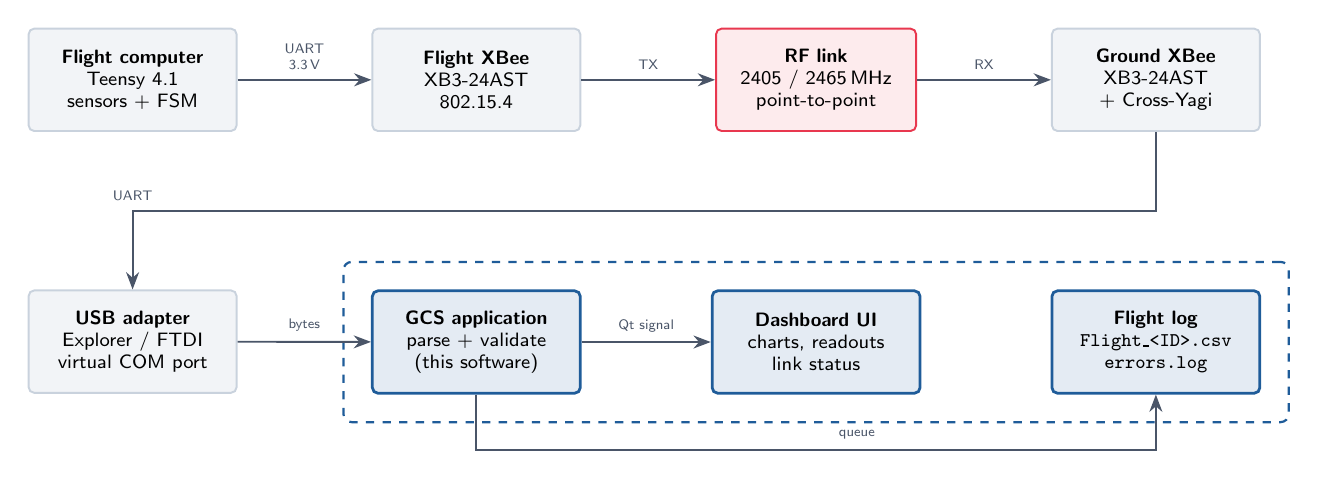
\begin{tikzpicture}[
  font=\sffamily\scriptsize,
  node distance=6mm,
  box/.style   ={draw=gcsrule, fill=gcslight, rounded corners=2pt,
                 minimum height=13mm, text width=25mm, align=center,
                 inner sep=2pt, line width=0.7pt},
  gcsbox/.style={draw=gcsblue, fill=gcsblue!12, rounded corners=2pt,
                 minimum height=13mm, text width=25mm, align=center,
                 inner sep=2pt, line width=1pt},
  rf/.style    ={draw=fsmDeploy, fill=fsmDeploy!10, rounded corners=2pt,
                 minimum height=13mm, text width=24mm, align=center,
                 inner sep=2pt, line width=0.7pt},
  ar/.style    ={-{Stealth[length=2.2mm]}, line width=0.7pt, draw=gcsgrey},
  lbl/.style   ={font=\sffamily\tiny, text=gcsgrey, midway, above, align=center},
  lblb/.style  ={font=\sffamily\tiny, text=gcsgrey, midway, below, align=center},
]

\node[box]                       (teensy) {\textbf{Flight computer}\\Teensy 4.1\\sensors + FSM};
\node[box,   right=17mm of teensy] (xbtx) {\textbf{Flight XBee}\\XB3-24AST\\802.15.4};
\node[rf,    right=17mm of xbtx]   (rf)   {\textbf{RF link}\\2405 / 2465\,MHz\\point-to-point};
\node[box,   right=17mm of rf]     (xbrx) {\textbf{Ground XBee}\\XB3-24AST\\+ Cross-Yagi};

\node[gcsbox, below=20mm of xbtx]  (gcs)  {\textbf{GCS application}\\parse + validate\\(this software)};
\node[gcsbox, below=20mm of rf]    (ui)   {\textbf{Dashboard UI}\\charts, readouts\\link status};
\node[gcsbox, below=20mm of xbrx]  (csv)  {\textbf{Flight log}\\\file{Flight\_<ID>.csv}\\\file{errors.log}};
\node[box,    below=20mm of teensy](usb)  {\textbf{USB adapter}\\Explorer / FTDI\\virtual COM port};

\draw[ar] (teensy) -- (xbtx) node[lbl]{UART\\3.3\,V};
\draw[ar] (xbtx)   -- (rf)   node[lbl]{TX};
\draw[ar] (rf)     -- (xbrx) node[lbl]{RX};
% Ground XBee drops down and runs left into the USB adapter.  The label sits on
% the horizontal leg (pos 0.5) so it cannot collide with either arrowhead.
\draw[ar] (xbrx.south) -- ++(0,-10mm) -| (usb.north) node[lbl,pos=0.5]{UART};
\draw[ar] (usb)    -- (gcs)  node[lbl]{bytes};
\draw[ar] (gcs)    -- (ui)   node[lbl]{Qt signal};
% Queue hand-off routed well below the row so it clears the dashed group box.
\draw[ar] (gcs.south) -- ++(0,-7mm) -| (csv.south) node[lbl,pos=0.28,above]{queue};

\begin{scope}[on background layer]
  % No label on the group box: the figure caption already identifies the
  % dashed region, and a label here collides with the queue arrow.
  \node[draw=gcsblue, dashed, rounded corners=3pt, line width=0.8pt,
        fit=(gcs)(ui)(csv), inner sep=3.5mm] {};
\end{scope}
\end{tikzpicture}
\caption{End-to-end telemetry chain. The GCS software covers the dashed
region: everything from raw serial bytes to the archived flight log.}
\label{fig:sysarch}
\end{figure}

\subsection{RF link parameters}

Both vehicles use the Digi XBee~3 PRO (XB3-24AST) operating under
IEEE~802.15.4 in point-to-point mode. Mesh/DigiMesh networking is
\emph{not} used: a single coordinator-to-endpoint association keeps latency
deterministic and removes routing overhead from a link that carries a
continuous 20\,Hz stream.

In the 2.4\,GHz 802.15.4 band, channel centre frequencies follow
\begin{equation}
f_c = 2405 + 5\,(k - 11)\ \text{MHz}, \qquad k = 11 \ldots 26,
\end{equation}
so the two mission frequencies map onto the XBee \param{CH} parameter as shown
in Table~\ref{tab:rf}. The \param{CH} register is set in hexadecimal in XCTU.

\begin{table}[htbp]
\centering
\caption{RF configuration per vehicle.}
\label{tab:rf}
\small
\begin{tabular}{@{}lccl@{}}
\toprule
\textbf{Vehicle} & \textbf{Frequency} & \textbf{802.15.4 channel (\param{CH})} & \textbf{Allocation}\\
\midrule
CanSat  & 2465\,MHz & 23 (\code{0x17}) & IN-SPACe channel assignment\\
Rocket  & 2405\,MHz & 11 (\code{0x0B}) & IN-SPACe channel assignment\\
\bottomrule
\end{tabular}
\end{table}

\critical{Both radios in a pair must match on three parameters}{The flight
unit and the ground unit must agree on \param{CH} (channel), \param{ID} (PAN
ID) and \param{BD} (serial baud rate). A mismatch on \param{CH} or \param{ID}
produces \emph{complete silence} with no error message anywhere --- the
dashboard will simply show \textsf{AWAITING TELEMETRY} forever. This is by
far the most common cause of a dead link on the bench, and the first thing to
check in the field. See Section~\ref{sec:hardware}.}

%==============================================================================
\section{Telemetry Packet Format}
\label{sec:packet}
%==============================================================================

\subsection{Frame structure}

Telemetry is transmitted as a single line of printable ASCII per sample:

\begin{center}
\fcolorbox{gcsrule}{gcslight}{%
\begin{minipage}{0.95\textwidth}
\ttfamily\footnotesize
\$TEAM\_ID,TIMESTAMP,PACKET\_COUNT,ALTITUDE,PRESSURE,TEMP,VOLTAGE,NAV\_TIME,\\
\hspace*{1em}LAT,LON,NAV\_ALT,SATS,ACC\_X,ACC\_Y,ACC\_Z,GYRO\_X,GYRO\_Y,GYRO\_Z,FSM\_STATE*CS
\end{minipage}}
\end{center}

The structure follows NMEA-0183 convention:

\begin{itemize}
  \item \code{\$} --- start delimiter, one byte (\code{0x24}). Marks the
        beginning of a frame.
  \item \emph{body} --- exactly 19 comma-separated fields. The body must not
        itself contain \code{\$} or \code{*}.
  \item \code{*} --- end delimiter, one byte (\code{0x2A}).
  \item \code{CS} --- exactly two uppercase or lowercase hexadecimal digits
        holding the XOR checksum of the body.
\end{itemize}

A trailing \code{CR\,LF} is optional; the parser tolerates its presence or
absence, and any bytes between the checksum and the next \code{\$} are
discarded as inter-frame junk.

A real frame, taken verbatim from the packet simulator, is:

\begin{center}
\fcolorbox{gcsrule}{white}{%
\begin{minipage}{0.95\textwidth}
\ttfamily\scriptsize
\$2025ASI001,0.05,2,320.04,975.39,25.90,8.20,012829.00,32.726600,\\
74.857001,317.81,4,-0.031,0.049,9.636,5.240,-1.444,1.506,0*43
\end{minipage}}
\end{center}

This frame is 125 bytes long, or 127 bytes with \code{CR\,LF}. That number
drives the link budget in Section~\ref{sec:baudbudget} and it is worth
remembering.

\subsection{Field definitions}

Table~\ref{tab:fields} defines all 19 fields. The \emph{Strictness} column
records how \file{telemetry\_packet.py} treats a blank or unparseable value:

\begin{description}[leftmargin=18mm,style=nextline,font=\normalfont\bfseries]
  \item[Mandatory] A blank or non-numeric value raises
        \code{PacketParseError} and the \emph{entire packet is rejected}.
        These are the fields without which the packet has no meaning.
  \item[Optional] A blank or non-numeric value is substituted with
        \code{NaN} (or \code{0} for integer counts) and the packet is
        \emph{still accepted}. This exists because a GNSS receiver
        legitimately transmits empty position fields before it achieves a
        fix; discarding those packets would blind the operator to altitude
        and flight state during the most critical part of the mission.
\end{description}

\begin{table}[htbp]
\centering
\caption{Telemetry field definitions, units and expected ranges.}
\label{tab:fields}
\scriptsize
\setlength{\tabcolsep}{4pt}
\renewcommand{\arraystretch}{1.15}
\begin{tabularx}{\textwidth}{@{}clllcX@{}}
\toprule
\textbf{\#} & \textbf{Field} & \textbf{Type} & \textbf{Unit} & \textbf{Strictness} & \textbf{Expected range / notes}\\
\midrule
1  & \code{TEAM\_ID}      & string & ---      & Mandatory & Competition team identifier, e.g.\ \code{2025ASI001}. Must be non-empty. Determines the CSV file name.\\
2  & \code{TIMESTAMP}     & float  & s        & Mandatory & Mission time since flight-computer boot, $0$--$7200$. Also accepts \code{HH:MM:SS} form. Drives the chart $x$-axis.\\
3  & \code{PACKET\_COUNT} & int    & ---      & Mandatory & Monotonically increasing from 1. Gaps indicate lost packets.\\
4  & \code{ALTITUDE}      & float  & m        & Mandatory & Barometric altitude. $-100$ to $15\,000$. MSL or AGL by firmware convention --- state which in the flight software ICD.\\
5  & \code{PRESSURE}      & float  & hPa      & Mandatory & Static pressure, $10$--$1100$. $\approx 1013.25$ at sea level.\\
6  & \code{TEMP}          & float  & \degC    & Mandatory & Ambient/board temperature, $-40$ to $+85$.\\
7  & \code{VOLTAGE}       & float  & V        & Mandatory & Battery bus voltage, $0$--$16$. Nominal $7.4$--$8.4$ for 2S Li-Po. Colour-coded against a configurable threshold.\\
8  & \code{NAV\_TIME}     & string & UTC      & Optional  & GNSS time as \code{hhmmss.ss}. May be blank before fix.\\
9  & \code{LAT}           & float  & deg      & Optional  & $-90$ to $+90$, positive north. Blank or $0,0$ treated as ``no fix''.\\
10 & \code{LON}           & float  & deg      & Optional  & $-180$ to $+180$, positive east.\\
11 & \code{NAV\_ALT}      & float  & m        & Optional  & GNSS altitude. Compare against field 4 as a barometer sanity check.\\
12 & \code{SATS}          & int    & count    & Optional  & Satellites in solution, $0$--$32$. Blank becomes $0$. UI warns below 6, alerts below 4.\\
13 & \code{ACC\_X}        & float  & m/s$^2$  & Optional  & Body-axis acceleration. $\pm157$ for a $\pm16$\,g IMU.\\
14 & \code{ACC\_Y}        & float  & m/s$^2$  & Optional  & As above.\\
15 & \code{ACC\_Z}        & float  & m/s$^2$  & Optional  & As above. $\approx +9.81$ at rest, vertical axis.\\
16 & \code{GYRO\_X}       & float  & deg/s    & Optional  & Body-axis angular rate, $\pm2000$.\\
17 & \code{GYRO\_Y}       & float  & deg/s    & Optional  & As above.\\
18 & \code{GYRO\_Z}       & float  & deg/s    & Optional  & As above. Roll/spin rate about the long axis.\\
19 & \code{FSM\_STATE}    & int    & enum     & Mandatory & Flight state, $0$--$7$. See Table~\ref{tab:fsm}. Out-of-range values display as \textsf{UNKNOWN} rather than being rejected.\\
\bottomrule
\end{tabularx}
\end{table}

\critical{Field count is fixed at 19}{The parser rejects any frame whose body
does not split into exactly 19 comma-separated fields. If the flight firmware
adds a field, \code{FIELD\_COUNT} in \file{telemetry\_packet.py} and
\code{CSV\_HEADER} must both be updated, and every previously recorded CSV
becomes a different schema. Version the packet format explicitly if this is
ever likely.}

\subsection{XOR checksum}
\label{sec:checksum}

The checksum is the bitwise exclusive-OR of every byte strictly between the
\code{\$} and the \code{*}, transmitted as two hexadecimal digits:
\begin{equation}
\text{CS} \;=\; b_1 \oplus b_2 \oplus \cdots \oplus b_n, \qquad
b_i = \text{ASCII byte } i \text{ of the body}.
\end{equation}

The implementation is deliberately trivial so that it can be reproduced
identically in the Teensy firmware:

\begin{lstlisting}[caption={XOR checksum, from \file{telemetry\_packet.py}.},label={lst:checksum}]
def compute_checksum(payload: str) -> int:
    """XOR every byte of *payload* (the text between ``$`` and ``*``)."""
    checksum = 0
    for byte in payload.encode("ascii", errors="replace"):
        checksum ^= byte
    return checksum & 0xFF
\end{lstlisting}

\subsubsection*{Worked example}

Take the trivial body \code{ABC}. The three ASCII bytes are XORed in
sequence:

\begin{table}[htbp]
\centering
\caption{Worked XOR checksum for the body \texttt{ABC}.}
\label{tab:xor}
\small
\begin{tabular}{@{}llll@{}}
\toprule
\textbf{Step} & \textbf{Character} & \textbf{Hex} & \textbf{Binary}\\
\midrule
Start           & ---        & \code{0x00} & \code{0000 0000}\\
$\oplus$ byte 1 & \code{A}   & \code{0x41} & \code{0100 0001}\\
$\oplus$ byte 2 & \code{B}   & \code{0x42} & \code{0100 0010}\\
$\oplus$ byte 3 & \code{C}   & \code{0x43} & \code{0100 0011}\\
\midrule
\textbf{Result} & \textbf{CS} & \textbf{\code{0x40}} & \textbf{\code{0100 0000}}\\
\bottomrule
\end{tabular}
\end{table}

Working it through: $0\text{x}00 \oplus 0\text{x}41 = 0\text{x}41$; then
$0\text{x}41 \oplus 0\text{x}42 = 0\text{x}03$; then
$0\text{x}03 \oplus 0\text{x}43 = 0\text{x}40$. The complete frame is
therefore \code{\$ABC*40}.

Note the checksum's properties and limits: XOR detects all single-byte errors
and any odd number of bit flips in a given bit position, but it does
\emph{not} detect a pair of identical bit flips in the same bit position of
two different bytes, nor does it detect transposed bytes. It is adequate for
catching the RF bit errors this link produces, and it is what the competition
format specifies, but it is not a CRC and should not be described as one.

\subsection{Flight state machine}

\code{FSM\_STATE} is an integer enumerating the flight computer's state. The
dashboard renders it as a large banner filled with a distinct colour per
state, so the operator can read the vehicle's state across a field tent at a
glance. The colours in Table~\ref{tab:fsm} are the exact values from
\code{FSM\_COLORS}.

\begin{table}[htbp]
\centering
\caption{Flight state machine states and dashboard colour coding.}
\label{tab:fsm}
\small
\begin{tabular}{@{}clllp{62mm}@{}}
\toprule
\textbf{Value} & \textbf{Name} & \textbf{Colour} & \textbf{Hex} & \textbf{Meaning}\\
\midrule
0 & \code{BOOT}              & \swatch{fsmBoot}      & \code{\#6B7785} & Power-on self-test; sensors initialising. Altitude not yet valid.\\
1 & \code{TEST\_MODE}        & \swatch{fsmTest}      & \code{\#00B0D8} & Bench/integration mode. Telemetry is live but the vehicle is not flight-armed.\\
2 & \code{LAUNCH\_PAD}       & \swatch{fsmPad}       & \code{\#E9C135} & Armed and on the pad. Ground reference pressure captured; awaiting launch detection.\\
3 & \code{ASCENT}            & \swatch{fsmAscent}    & \code{\#F07419} & Launch detected; powered and coast ascent to apogee.\\
4 & \code{DEPLOY}            & \swatch{fsmDeploy}    & \code{\#E8384F} & Apogee detected; recovery deployment event commanded.\\
5 & \code{DESCENT}           & \swatch{fsmDescent}   & \code{\#8F6BEF} & Descending under the primary recovery device.\\
6 & \code{AEROBRAKE\_RELEASE}& \swatch{fsmAerobrake} & \code{\#00B39B} & Aerobrake / main recovery released; reduced descent rate.\\
7 & \code{IMPACT}            & \swatch{fsmImpact}    & \code{\#35C46B} & Touchdown detected; vehicle stationary on the ground.\\
\bottomrule
\end{tabular}
\end{table}

Every state \emph{transition} is timestamped into the on-screen event log, in
the form \code{FSM ASCENT -> DEPLOY at T+00:00:24}, which gives a
post-flight event timeline without needing to reprocess the CSV.

%==============================================================================
\section{Software Architecture}
\label{sec:arch}
%==============================================================================

\subsection{Module layout}

The application is six Python modules with a strict dependency direction:
nothing that touches hardware imports anything that touches widgets.

\begin{table}[htbp]
\centering
\caption{Source module responsibilities.}
\label{tab:modules}
\small
\begin{tabular}{@{}lrp{78mm}@{}}
\toprule
\textbf{Module} & \textbf{Lines} & \textbf{Responsibility}\\
\midrule
\file{main.py}              & $\sim$140 & Entry point, CLI arguments, exception hook.\\
\file{telemetry\_packet.py} & $\sim$400 & Packet dataclass, checksum, parser. No Qt.\\
\file{serial\_worker.py}    & $\sim$470 & Serial thread, ring buffer, frame sync, reconnect.\\
\file{csv\_logger.py}       & $\sim$300 & Logging thread, CSV and error files.\\
\file{dashboard\_ui.py}     & $\sim$1000& Main window, all widgets and plots.\\
\file{packet\_sim.py}       & $\sim$520 & Synthetic telemetry source and fault injector.\\
\bottomrule
\end{tabular}
\end{table}

\subsubsection{\file{telemetry\_packet.py} --- packet model and parser}

This is the foundation module and the only one with no dependencies on Qt,
pyserial or anything else. That property is deliberate: it means the parser
can be exercised by the fuzz harness, by unit tests and by the packet
simulator without constructing a \code{QApplication}, and it means the
simulator and the receiver share one definition of the wire format and can
therefore never drift apart.

\textbf{Key contents:}
\begin{itemize}
  \item \code{TelemetryPacket} --- a \code{@dataclass(slots=True)} holding all
        19 fields plus three ground-station annotations:
        \code{raw\_frame}, \code{checksum\_valid} and \code{gs\_recv\_epoch}.
        Derived properties (\code{fsm\_name}, \code{fsm\_color},
        \code{mission\_time\_hms}, \code{has\_fix}) keep formatting logic out
        of the UI.
  \item \code{compute\_checksum()} and \code{build\_frame()} --- the checksum
        pair, used by both the receiver and the simulator.
  \item \code{parse\_frame()} --- the single entry point that turns one frame
        string into a \code{TelemetryPacket} or raises.
  \item \code{CSV\_HEADER} --- the canonical column list, kept adjacent to
        \code{to\_csv\_row()} so the two cannot diverge.
  \item Exception hierarchy: \code{PacketError} is the base;
        \code{ChecksumError} means the link corrupted the frame;
        \code{PacketParseError} means the frame was structurally wrong. A
        caller that only cares ``was this usable'' catches the base class.
\end{itemize}

\begin{lstlisting}[caption={Packet validation flow, from \code{parse\_frame()}.},label={lst:parse}]
    match = _FRAME_RE.match(text)
    if match is None:
        raise PacketParseError("frame does not match $<body>*<hh>: %r" % text[:120])

    body = match.group("body")
    transmitted = int(match.group("cs"), 16)

    calculated = compute_checksum(body)
    if calculated != transmitted:
        raise ChecksumError(
            "checksum mismatch: got %02X, expected %02X" % (transmitted, calculated)
        )

    fields = body.split(",")
    if len(fields) != FIELD_COUNT:
        raise PacketParseError(
            "expected %d fields, got %d" % (FIELD_COUNT, len(fields))
        )
\end{lstlisting}

\subsubsection{\file{serial\_worker.py} --- ingestion thread}

Owns the pyserial handle and everything that happens to bytes before they
become packets. Contains three classes:

\begin{itemize}
  \item \code{RingBuffer} --- a fixed-capacity, drop-oldest byte buffer
        (8192\,bytes) that bounds memory even if the stream is pure garbage.
  \item \code{FrameSplitter} --- the frame-sync state machine
        (Section~\ref{sec:framesync}).
  \item \code{SerialWorker(QThread)} --- the run loop: connect, read, split,
        parse, emit, reconnect.
\end{itemize}

\code{SerialWorker} exposes its results exclusively through Qt signals, which
Qt delivers to the GUI thread through a queued connection automatically:

\begin{lstlisting}[caption={\code{SerialWorker} signal interface.},label={lst:signals}]
    packet_received = pyqtSignal(object)          # a validated TelemetryPacket
    bad_frame = pyqtSignal(str, str)              # (raw_frame_text, reason)
    stats_updated = pyqtSignal(int, int, int)     # (total, valid, corrupt)
    connection_changed = pyqtSignal(bool, str)    # (is_connected, message)
    log_message = pyqtSignal(str)                 # free-form event log line
\end{lstlisting}

The thread is \emph{long-lived}. It starts once at application launch and
stops once at exit. Pressing \textsf{CONNECT} or \textsf{DISCONNECT} does not
start or stop the thread; it flips a \code{\_want\_connected} flag guarded by
a \code{threading.Lock} that the run loop watches. This is what makes
automatic reconnection free: if the USB adapter is unplugged mid-flight, the
read raises, the loop closes the handle and keeps retrying every 1.5\,s until
the port reappears --- with no operator action and no risk of the application
dying.

Statistics emission is throttled to 5\,Hz. Emitting a signal per packet
during a burst would flood the GUI event loop with thousands of queued
events, which is precisely the failure mode this architecture exists to
prevent.

\subsubsection{\file{csv\_logger.py} --- disk logging thread}

A \code{QThread} that consumes a \code{queue.Queue} and writes two files.
Disk I/O is kept off both the GUI thread (where a stalled write would freeze
the display) and the serial thread (where it would cause the driver's receive
buffer to overflow and lose packets).

\code{queue.Queue} is used rather than a Qt signal because this is a plain
producer/consumer handoff with no Qt object affinity involved, and because a
\emph{bounded} queue gives explicit back-pressure semantics. If the disk
stalls, the oldest rows are dropped and counted, rather than the producer
blocking:

\begin{lstlisting}[caption={Non-blocking, never-raising enqueue, from \file{csv\_logger.py}.},label={lst:queue}]
    def _put(self, item: Tuple[str, Any]) -> None:
        try:
            self._queue.put_nowait(item)
        except queue.Full:
            # Back-pressure: drop the oldest item so live data keeps flowing.
            try:
                self._queue.get_nowait()
                self.rows_dropped += 1
                self._queue.put_nowait(item)
            except (queue.Empty, queue.Full):
                self.rows_dropped += 1
\end{lstlisting}

Two behaviours are worth knowing:

\begin{itemize}
  \item \textbf{Lazy file open.} The CSV cannot be named until
        \code{TEAM\_ID} is known, so the file is opened on the first packet
        received, not when logging is enabled.
  \item \textbf{Append, never truncate.} \file{Flight\_<TEAM\_ID>.csv} is
        opened in append mode and the header is written only when the file is
        new or empty. A mid-competition application restart therefore cannot
        destroy the earlier part of the flight.
  \item \textbf{Flush policy.} The writer flushes at least every 20 rows and
        at least every 1\,second, so a crash costs a fraction of a second of
        telemetry. A full \code{os.fsync} is performed only at clean shutdown;
        calling it at 20\,Hz would thrash the disk for no benefit against the
        realistic failure mode, which is a process crash rather than a power
        loss on the laptop.
\end{itemize}

\subsubsection{\file{dashboard\_ui.py} --- main window}

Contains every widget and owns both worker threads. The important classes:

\begin{itemize}
  \item \code{ReadoutTile} --- a labelled numeric tile with normal / ok /
        warn / alert colour states.
  \item \code{StripChart} --- a \code{pg.PlotWidget} subclass that holds its
        own data buffers and separates \code{add\_point()} (cheap, per packet)
        from \code{redraw()} (timer-driven).
  \item \code{GpsTrackPlot} --- the lat/lon ground track.
  \item \code{Dashboard(QMainWindow)} --- layout, signal wiring, timers,
        connection and logging control, and clean shutdown.
\end{itemize}

\subsubsection{\file{main.py} --- entry point}

Sets the High-DPI attributes \emph{before} the \code{QApplication} is
constructed (Qt ignores them afterwards), applies the dark palette, parses
\code{--port}, \code{--baud}, \code{--autoconnect} and \code{--log-dir}, and
installs a \code{sys.excepthook} that routes an uncaught GUI-thread exception
into the on-screen event log and the error file instead of killing the
process. A display bug must not end a flight.

\subsubsection{\file{packet\_sim.py} --- synthetic source}

Not part of the flight-day software, but part of the deliverable: it flies a
scripted mission and emits real checksum-correct frames so the whole chain can
be exercised without a radio. Covered in Section~\ref{sec:testing}.

\subsection{Threading model}
\label{sec:threading}

The application runs exactly three threads, shown in
Figure~\ref{fig:threads}.

\begin{figure}[htbp]
\centering
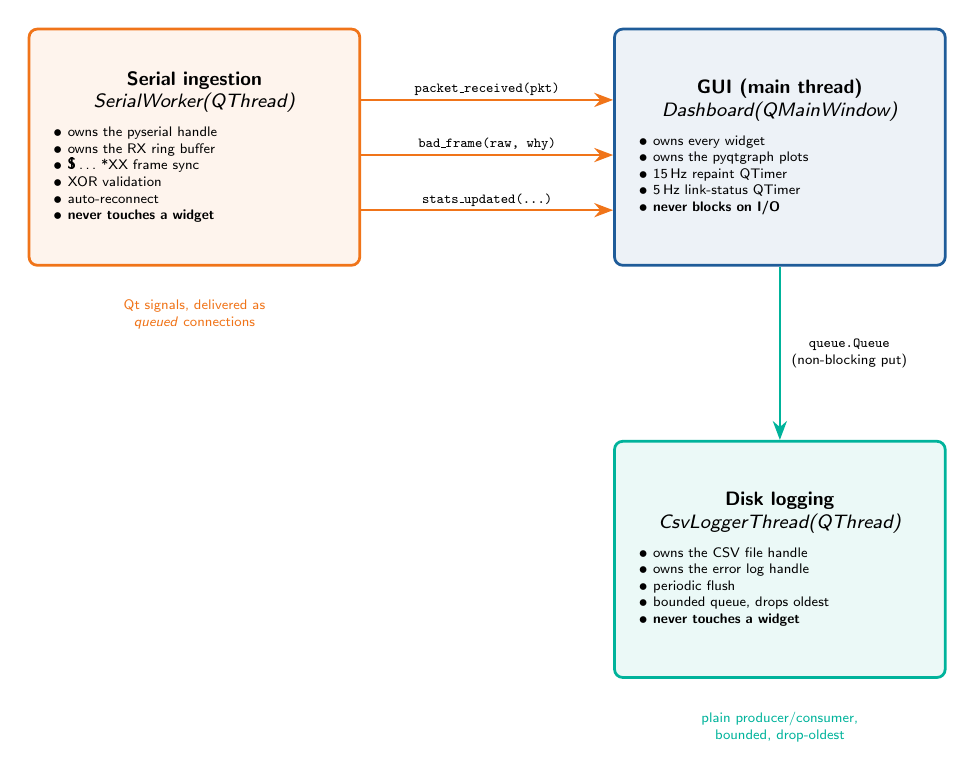
\begin{tikzpicture}[
  font=\sffamily\scriptsize,
  th/.style   ={draw, rounded corners=3pt, minimum width=42mm,
                minimum height=30mm, align=center, inner sep=3mm,
                line width=1pt},
  ser/.style  ={th, draw=fsmAscent,  fill=fsmAscent!8},
  gui/.style  ={th, draw=gcsblue,    fill=gcsblue!8},
  log/.style  ={th, draw=fsmAerobrake, fill=fsmAerobrake!8},
  ar/.style   ={-{Stealth[length=2.4mm]}, line width=0.9pt},
  lbl/.style  ={font=\sffamily\tiny, align=center, fill=white, inner sep=1pt},
]

\node[ser] (s) {%
  \textbf{Serial ingestion}\\\textit{SerialWorker(QThread)}\\[1.5mm]
  \footnotesize
  \begin{minipage}{36mm}\raggedright\tiny
  $\bullet$ owns the pyserial handle\\
  $\bullet$ owns the RX ring buffer\\
  $\bullet$ \$\,\ldots\,*XX frame sync\\
  $\bullet$ XOR validation\\
  $\bullet$ auto-reconnect\\
  $\bullet$ \textbf{never touches a widget}
  \end{minipage}};

\node[gui, right=32mm of s] (g) {%
  \textbf{GUI (main thread)}\\\textit{Dashboard(QMainWindow)}\\[1.5mm]
  \begin{minipage}{36mm}\raggedright\tiny
  $\bullet$ owns every widget\\
  $\bullet$ owns the pyqtgraph plots\\
  $\bullet$ 15\,Hz repaint QTimer\\
  $\bullet$ 5\,Hz link-status QTimer\\
  $\bullet$ \textbf{never blocks on I/O}
  \end{minipage}};

\node[log, below=22mm of g] (l) {%
  \textbf{Disk logging}\\\textit{CsvLoggerThread(QThread)}\\[1.5mm]
  \begin{minipage}{36mm}\raggedright\tiny
  $\bullet$ owns the CSV file handle\\
  $\bullet$ owns the error log handle\\
  $\bullet$ periodic flush\\
  $\bullet$ bounded queue, drops oldest\\
  $\bullet$ \textbf{never touches a widget}
  \end{minipage}};

\draw[ar, draw=fsmAscent] ([yshift=6mm]s.east) -- ([yshift=6mm]g.west)
  node[lbl, midway, above]{\texttt{packet\_received(pkt)}};
\draw[ar, draw=fsmAscent] ([yshift=-1mm]s.east) -- ([yshift=-1mm]g.west)
  node[lbl, midway, above]{\texttt{bad\_frame(raw, why)}};
\draw[ar, draw=fsmAscent] ([yshift=-8mm]s.east) -- ([yshift=-8mm]g.west)
  node[lbl, midway, above]{\texttt{stats\_updated(...)}};

\draw[ar, draw=fsmAerobrake] (g) -- (l)
  node[lbl, midway, right, xshift=1mm]{\texttt{queue.Queue}\\(non-blocking put)};

\node[below=3mm of s, font=\sffamily\tiny, text=fsmAscent, align=center]
  {Qt signals, delivered as\\\emph{queued} connections};
\node[below=3mm of l, font=\sffamily\tiny, text=fsmAerobrake, align=center]
  {plain producer/consumer,\\bounded, drop-oldest};

\end{tikzpicture}
\caption{Three-thread model. Ownership is exclusive: exactly one thread may
touch the serial port, exactly one may touch the log files, and exactly one
may touch widgets.}
\label{fig:threads}
\end{figure}

\subsubsection{Why serial I/O is not on the GUI thread}

A serial read is a blocking call. Every millisecond the GUI thread spends
inside \code{read()} is a millisecond it is not processing paint events,
button clicks or window messages. At 20\,Hz with a 50\,ms read timeout, a
single-threaded design would spend essentially all of its time blocked and
Windows would mark the window ``Not Responding''. Worse, the operator would
lose the ability to press \textsf{DISCONNECT} at exactly the moment something
had gone wrong.

\subsubsection{Why disk I/O is not on the GUI thread}

A write to a USB stick, a network drive or a disk that has decided to spin up
can block for hundreds of milliseconds. On the GUI thread that is a visible
freeze; on the serial thread it is worse, because while the thread is blocked
in \code{write()} it is not draining the driver's receive buffer, so packets
are lost on the floor. Moving the writes to a third thread means a slow disk
degrades to queued rows, not to lost telemetry.

\subsubsection{Render decoupling --- the reason the UI never freezes}

This is the single most important design decision in the application, and the
one most likely to be broken by a well-meaning future edit.

The \code{on\_packet} slot is deliberately cheap. It appends numbers to Python
lists, stores the latest packet, and sets a dirty flag. \textbf{It repaints
nothing.} All drawing happens in a separate \code{QTimer} callback running at
15\,Hz:

\begin{lstlisting}[caption={Timer-driven rendering, from \file{dashboard\_ui.py}.},label={lst:render}]
    def _render(self) -> None:
        """Repaint readouts and charts at a fixed rate, independent of RX rate."""
        try:
            if self._readouts_dirty:
                self._readouts_dirty = False
                self._update_readouts()

                window_s = float(self.window_spin.value())
                autoscale = self.autoscroll_check.isChecked()
                for chart in self.charts:
                    chart.redraw(window_s, autoscale)
                self.gps_plot.redraw()
        except Exception as exc:  # pragma: no cover - defensive
            self.append_event("Render error: %r" % exc)
\end{lstlisting}

The consequence: whether the radio delivers 5 packets per second or dumps a
500-packet backlog after a dropout, the number of repaints per second is
constant at 15. Repainting six pyqtgraph plots is the expensive operation in
this application; decoupling it from arrival rate is what satisfies the
``tolerate bursts without freezing'' requirement.

\critical{Do not repaint from \texttt{on\_packet}}{If a future change calls
\code{setData()}, \code{setText()} or any other widget method directly from
the \code{packet\_received} slot, the application will appear to work
perfectly at 10\,Hz on the bench and will lock solid the first time the link
recovers from a dropout and delivers a burst. Add data to the buffers; let the
timer draw.}

\subsection{Ring buffer and frame synchronisation}
\label{sec:framesync}

\subsubsection{The problem}

The serial stream is not frame-aligned. A single \code{read()} may return
half a packet, two and a half packets, or a packet with 40 bytes of RF noise
in front of it. The receiver must find packet boundaries in an arbitrary byte
stream, and must do so in a way that cannot be permanently derailed by any
input.

\subsubsection{The ring buffer}

Incoming bytes are appended to a \code{RingBuffer} of fixed 8192-byte
capacity --- roughly 64 full frames, or over 3 seconds of backlog at 20\,Hz,
far more than a healthy reader ever accumulates. When the buffer is full the
\emph{oldest} bytes are evicted and counted in \code{dropped\_bytes}. This
guarantees bounded memory: a stream of pure garbage, or a transmitter stuck
sending a continuous carrier, cannot grow the process without limit.

It is implemented over a \code{bytearray} with front-trimming rather than a
wrapped index pair, because the frame scanner needs \emph{contiguous} memory
to run \code{bytes.find()} over. The externally visible behaviour ---
fixed capacity, drop-oldest --- is what matters.

\subsubsection{The frame-sync rules}

\code{FrameSplitter.\_extract()} repeatedly applies three rules until no more
complete frames can be produced:

\begin{enumerate}
  \item \textbf{Discard leading junk.} Everything before the first \code{\$}
        is not part of any frame. Drop it. This is what silently absorbs RF
        noise, partial frames received before the receiver started, and ---
        as discussed in Section~\ref{sec:apimode} --- XBee API frame headers.
  \item \textbf{Restart on a second \code{\$}.} If another \code{\$} appears
        before the terminating \code{*}, the first frame was truncated in
        flight. Abandon it and restart parsing at the newer \code{\$}. Every
        such event increments a \code{resyncs} counter.
  \item \textbf{Bound the frame length.} If the buffer grows past
        \code{MAX\_FRAME\_LEN} (512 bytes) without producing a terminator,
        the leading \code{\$} is spurious. Drop that one byte and rescan.
        This rule is what prevents a lost \code{*} from wedging the reader
        forever.
\end{enumerate}

If none of the rules fire and the terminator simply has not arrived yet, the
scanner returns and waits for more bytes --- the partial frame stays in the
buffer across calls, which is what makes byte-at-a-time reassembly work.

\begin{lstlisting}[caption={Frame-sync loop, from \file{serial\_worker.py}.},label={lst:framesync}]
        while True:
            start = buf.find(b"$")
            if start < 0:
                # No frame start at all: the whole buffer is junk.
                buf.clear()
                break
            if start > 0:
                buf.consume(start)  # rule 1: drop leading junk

            star = buf.find(b"*", 1)
            next_dollar = buf.find(b"$", 1)

            if 0 <= next_dollar and (star < 0 or next_dollar < star):
                # rule 2: truncated frame, restart at the newer '$'
                buf.consume(next_dollar)
                self.resyncs += 1
                continue

            if star < 0:
                # Terminator has not arrived yet.
                if len(buf) > MAX_FRAME_LEN:
                    buf.consume(1)  # rule 3
                    self.resyncs += 1
                    continue
                break
\end{lstlisting}

\subsubsection{Worked recovery example}

Consider this hostile stream, which is exactly what the fault injector
produces:

\begin{center}
\ttfamily\footnotesize
\textcolor{gcsgrey}{qk3\$\%z9}\,\textcolor{fsmImpact}{\$TEAM,...,3*4A}\,\textbackslash r\textbackslash n\,\textcolor{fsmDeploy}{\$TEAM,12.5,88,}\,\textcolor{fsmImpact}{\$TEAM,...,4*7C}
\end{center}

\begin{enumerate}
  \item \textcolor{gcsgrey}{\texttt{qk3}} precedes the first \code{\$} ---
        discarded by rule~1. (The \code{\$} inside the junk becomes the
        candidate start; the following \code{\%z9} then fails rule~2 or the
        checksum, and is discarded.)
  \item \textcolor{fsmImpact}{The first complete frame} is found, checksum
        verified, emitted as a packet.
  \item \code{\textbackslash r\textbackslash n} precedes the next \code{\$}
        --- discarded by rule~1.
  \item \textcolor{fsmDeploy}{The truncated frame} has no \code{*} before the
        next \code{\$} --- abandoned by rule~2, \code{resyncs} incremented.
        No packet is emitted and nothing is corrupted.
  \item \textcolor{fsmImpact}{The final frame} parses normally.
\end{enumerate}

Net result: two valid packets recovered, one resync, zero exceptions, zero
false packets. This exact behaviour is verified by test \textbf{GCS-T-04} in
Section~\ref{sec:testing}.

\subsubsection{Three layers of defence}

The robustness requirement is met by three independent layers, so that a
failure of one does not reach the operator:

\begin{enumerate}
  \item \textbf{Structural} --- the frame-sync rules discard anything that
        does not look like a frame, without ever raising.
  \item \textbf{Cryptographic (weakly)} --- the XOR checksum rejects frames
        whose bytes were altered in flight. These are counted as
        \emph{corrupt} and shown in the link status panel.
  \item \textbf{Defensive} --- \code{\_handle\_frame()} wraps
        \code{parse\_frame()} in \code{try/except} that catches
        \code{ChecksumError}, \code{PacketParseError}, the \code{PacketError}
        base class \emph{and} bare \code{Exception}. A latent bug in the
        parser itself therefore costs one packet, not the ingestion thread:
\end{enumerate}

\begin{lstlisting}[caption={Catch-all in the ingestion path, from \file{serial\_worker.py}.},label={lst:catchall}]
        except Exception as exc:
            # A bug in the parser must not kill the ingestion thread mid-flight.
            self.corrupt_packets += 1
            self.bad_frame.emit(frame, "unexpected %s: %s" % (type(exc).__name__, exc))
            return
\end{lstlisting}

Every rejected frame, from any of the three layers, is forwarded to the error
log with its raw bytes and the reason --- unconditionally, even when CSV
logging is switched off, so that a post-flight link investigation always has
data.

%==============================================================================
\section{Dashboard UI Reference}
\label{sec:ui}
%==============================================================================

\subsection{Overall layout}

The window is organised as a connection bar across the top, a fixed-width
status column on the left, and a $3\times2$ grid of strip charts filling the
remainder. The theme is dark by design: the station is read outdoors and in a
field tent, where a white background is both glare-prone and a significant
battery drain on an LCD backlight.

\screenshot{dashboard_main.png}{Main dashboard during a simulated flight.
Left column: flight-state banner, live telemetry tiles, GPS/NavIC panel with
ground track, link status and display settings. Right: altitude, pressure,
temperature, battery voltage, accelerometer and gyroscope strip
charts.}{main}{1.0}

\subsection{Connection bar}

\begin{table}[htbp]
\centering
\caption{Connection bar controls.}
\label{tab:connbar}
\small
\begin{tabularx}{\textwidth}{@{}lX@{}}
\toprule
\textbf{Control} & \textbf{Function}\\
\midrule
\textsf{Port}          & Editable dropdown of detected serial devices. Also accepts a typed pyserial URL such as \code{socket://127.0.0.1:5555}. See Section~\ref{sec:comport}.\\
\textsf{RESCAN}        & Re-enumerates serial ports without restarting the application. Use after plugging in the XBee adapter.\\
\textsf{Baud}          & Editable baud selector, default 9600. Must match the radio's \param{BD} setting --- see Section~\ref{sec:baudbudget}.\\
\textsf{CONNECT}       & Opens the link. Turns red and reads \textsf{DISCONNECT} while connected.\\
\textsf{START LOGGING} & Toggles CSV writing. The error log is always written regardless of this setting.\\
\textsf{CSV: \ldots}   & Full path of the active flight log, shown once the first packet has arrived and the file name is known.\\
\textsf{CONNECTED}     & Link indicator: green when the port is open, red when it is not.\\
\bottomrule
\end{tabularx}
\end{table}

\subsection{Flight state banner and live telemetry}

The banner fills with the state colour from Table~\ref{tab:fsm} and shows the
state name and numeric value, e.g.\ \textsf{DESCENT~[5]}. It is pinned above
the scrolling region so it can never be scrolled out of view on a short
laptop screen.

Below it, eight tiles show Team ID, Packet Count, Mission Time
(\code{HH:MM:SS}), Altitude, Pressure, Temperature, Battery and Satellites.
Two tiles are colour-coded:

\begin{itemize}
  \item \textbf{Battery} --- green at or above the configurable threshold
        (default 7.00\,V), amber below it, red below 90\,\% of it. The
        threshold is set in the Display Settings panel and should be set to
        the flight computer's brown-out margin, not to an arbitrary round
        number.
  \item \textbf{Satellites} --- green at 6 or more, amber at 4--5, red below
        4. Below 4 satellites there is no 3D position solution at all.
\end{itemize}

A field showing \code{--} means the flight computer transmitted a blank or
unparseable value for an \emph{optional} field; the rest of the packet is
still valid and still logged.

\subsection{Strip charts}

Six pyqtgraph plots share a common $x$-axis definition: mission time in
seconds, taken from the packet \code{TIMESTAMP} field, falling back to
ground-station elapsed time if the flight computer sends a timestamp that
cannot be interpreted.

\begin{table}[htbp]
\centering
\caption{Strip chart contents.}
\label{tab:charts}
\small
\begin{tabularx}{\textwidth}{@{}llX@{}}
\toprule
\textbf{Chart} & \textbf{Series} & \textbf{What to look for}\\
\midrule
Altitude        & 1 (blue)   & The flight profile. Should be monotonic up to apogee, then monotonic down. Steps or spikes indicate barometer noise or a pressure-port problem.\\
Pressure        & 1 (orange) & The mirror image of altitude. If altitude moves and pressure does not, the altitude is being computed from a stale reading.\\
Temperature     & 1 (red)    & Should fall with altitude at roughly 6.5\,\degC{} per 1000\,m. A rise during ascent suggests self-heating or a sensor near the electronics.\\
Battery voltage & 1 (green)  & Slow droop is normal. A sharp sag correlated with a deployment event indicates the recovery charge is loading the same bus as the avionics.\\
Accelerometer   & 3 (X/Y/Z)  & $\approx +9.81$\,m/s$^2$ on the vertical axis at rest. The launch transient and the deployment shock should both be clearly visible.\\
Gyroscope       & 3 (X/Y/Z)  & Roll rate about the long axis. A high, non-decaying spin rate under the recovery device indicates a tangled or asymmetric deployment.\\
\bottomrule
\end{tabularx}
\end{table}

The visible time window is set by \textsf{Chart window (s)} in Display
Settings, default 60\,s, range 5--1800\,s. Charts are pannable and zoomable
with the mouse; unticking \textsf{Auto-scale Y axes} freezes the vertical
range so a manually chosen scale is not overridden.

\subsection{GPS / NavIC panel}

\screenshot{gps_panel.png}{GPS/NavIC panel: latitude, longitude, navigation
altitude and navigation time readouts above the two-dimensional ground
track.}{gps}{0.55}

The four readouts show \code{LAT}, \code{LON}, \code{NAV\_ALT} and
\code{NAV\_TIME}. Latitude and longitude turn amber when the packet does not
carry a usable fix --- either the fields were blank, or they contained the
$0,0$ null-island default that many receivers emit before lock.

The ground track plots longitude on $x$ against latitude on $y$: a faint blue
path of every fix received in the session, with a red crosshair marking the
most recent one. Note that this is a plain Cartesian scatter, not a
georeferenced map --- see Section~\ref{sec:limitations}. For recovery
purposes, read the numeric latitude and longitude, not the plot.

\subsection{Link status panel}

\screenshot{link_status.png}{Link status panel showing packet rate, last
packet age, valid/total packet counts, corrupt packet count and the link
health banner.}{link}{0.55}

This panel is the operator's primary health indicator for the RF link.

\begin{table}[htbp]
\centering
\caption{Link status fields.}
\label{tab:linkstatus}
\small
\begin{tabularx}{\textwidth}{@{}lX@{}}
\toprule
\textbf{Field} & \textbf{Meaning and interpretation}\\
\midrule
\textsf{Packet rate}      & Valid packets per second, averaged over a trailing 3-second window. Should sit near the firmware's transmit rate. A rate well below it means packets are being lost on the RF link or the serial line is oversubscribed (Section~\ref{sec:baudbudget}).\\
\textsf{Last packet age}  & Seconds since the last \emph{valid} packet. Green under 2\,s, red above.\\
\textsf{Valid / total pkts} & Valid packets over total frames recovered from the stream. The difference is the number rejected. A widening gap is the earliest warning of a degrading link.\\
\textsf{Corrupt packets}  & Frames that were structurally complete but failed checksum or parsing. Turns red as soon as it is non-zero. A handful over a flight is normal; a steadily climbing count means the link is marginal.\\
\textsf{Health banner}    & \textsf{AWAITING TELEMETRY} before the first packet, \textsf{LINK NOMINAL} in green while healthy, \textsf{!! TELEMETRY STALE !!} in red after 2\,s without a valid packet.\\
\bottomrule
\end{tabularx}
\end{table}

Every stale/recovered transition is also written to the event log and the
error log with a timestamp, giving a dropout record for post-flight analysis.

\subsection{Display settings and event log}

\textsf{Chart window (s)}, \textsf{Battery warning (V)} and
\textsf{Auto-scale Y axes} are described above. \textsf{Clear plots \&
counters} wipes the on-screen history and zeroes the counters; it does
\emph{not} touch the CSV, which continues uninterrupted.

The event log at the bottom of the column carries timestamped entries for
connections, disconnections, port errors, FSM transitions, stale/recovered
events and logging start/stop. The most recent entry is mirrored in the
status bar at the bottom of the window.

%==============================================================================
\section{Testing and Validation Performed}
\label{sec:testing}
%==============================================================================

\subsection{Approach}

Verification was performed at three levels: pure-logic tests against the
parser and framer with no Qt involved; integration tests running the real
\code{Dashboard} with real worker threads against a real socket, driven
offscreen; and a windowed visual check. All tests ran against the delivered
source, on Python 3.11 with PyQt5 5.15.11, pyqtgraph 0.14.0 and pyserial 3.5.

\subsection{Test matrix}

% First column is wide enough to hold "GCS-T-01" on one line; at 16mm it broke
% at the internal hyphens and read as two lines.
\begin{longtable}{@{}p{21mm}L{50mm}L{53mm}p{15mm}@{}}
\caption{Ground station verification test matrix.}\label{tab:testmatrix}\\
\toprule
\textbf{Test ID} & \textbf{Method} & \textbf{Result observed} & \textbf{Verdict}\\
\midrule
\endfirsthead
\multicolumn{4}{@{}l}{\small\itshape Table~\ref{tab:testmatrix} continued from previous page}\\
\toprule
\textbf{Test ID} & \textbf{Method} & \textbf{Result observed} & \textbf{Verdict}\\
\midrule
\endhead
\midrule
\multicolumn{4}{r@{}}{\small\itshape continued on next page}\\
\endfoot
\bottomrule
\endlastfoot

GCS-T-01 & Build a frame with \code{build\_frame()}, parse it back with \code{parse\_frame()}; compare all 19 fields. & All fields recovered exactly; \code{ASCENT} resolved from state 3; mission time rendered \code{00:00:12}; CSV row length equals \code{CSV\_HEADER} length. & \textbf{PASS}\\

GCS-T-02 & Corrupt the two checksum digits of a valid frame and parse. & \code{ChecksumError} raised; frame rejected, not displayed. & \textbf{PASS}\\

GCS-T-03 & Parser fuzz: 4013 malformed inputs --- empty strings, bare delimiters, 600-char frames, doubled frames, truncated frames, \code{NaN} fields, and random byte strings drawn from an alphabet including \code{NUL} and \code{0xFF}. & Zero unexpected exceptions. Every input either parsed or raised a \code{PacketError} subclass. No crash, no hang. & \textbf{PASS}\\

GCS-T-04 & Frame sync: a stream of leading garbage, one good frame, one truncated frame with no terminator, a second good frame and a third with no trailing \code{CRLF}, fed \textbf{one byte at a time}. & All 3 good frames recovered and parsed; 1 resync recorded on the truncated frame; no false packets emitted. & \textbf{PASS}\\

GCS-T-05 & Ring buffer bound: feed 200\,000 bytes of non-frame data. & Buffer held at 8192 bytes; 283\,747 bytes counted as dropped across the test; memory bounded. & \textbf{PASS}\\

GCS-T-06 & Wedge resistance: feed \code{\$} followed by 100\,000 bytes with no terminator, then a valid frame. & Rule 3 forced resync; the subsequent valid frame was still recovered. Reader did not wedge. & \textbf{PASS}\\

GCS-T-07 & Simulator coverage: sample the mission profile across the full timeline and parse every frame. & All frames valid; all 8 FSM states $\{0\ldots7\}$ produced, confirming full state coverage for UI testing. & \textbf{PASS}\\

GCS-T-08 & Fault-injected stream: 3000 frames at 15\,\% corrupt, 15\,\% garbage-prefixed, 15\,\% truncated, 10\,\% dropped, through the real framer and parser. & 1909 valid packets recovered, 362 checksum failures correctly detected, 0 malformed escapes, 425 resyncs. No unexpected exception. & \textbf{PASS}\\

GCS-T-09 & Live integration: real \code{Dashboard}, real \code{SerialWorker} and \code{CsvLoggerThread}, real TCP socket, simulator at 20\,Hz in \code{--chaos} mode, 16-second run. & 259 valid packets, 16 corrupt correctly rejected, 275 total frames. Readouts, all six charts and the ground track updated live. & \textbf{PASS}\\

GCS-T-10 & GUI responsiveness under burst: independent 50\,ms watchdog timer during GCS-T-09, including a 40-packet burst after 3\,s of silence. & Watchdog fired continuously throughout; event loop never blocked; no ``Not Responding'' state. & \textbf{PASS}\\

GCS-T-11 & Stale-link detection: observe the banner across the simulator's 3-second silence gap. & Banner switched to \textsf{TELEMETRY STALE} after 2\,s, logged the transition, and returned to \textsf{LINK NOMINAL} on recovery, logging that too. & \textbf{PASS}\\

GCS-T-12 & Auto-reconnect, four transitions: (a) connect with no peer present; (b) start the peer; (c) kill the peer mid-stream; (d) restart the peer. & (a) retried without crashing, connected=False; (b) auto-connected, 94 packets; (c) loss detected, connected=False; (d) auto-recovered to 212 packets. No operator action at any step. & \textbf{PASS}\\

GCS-T-13 & Clean shutdown and CSV integrity: close the window during an active logging session, then inspect the file. & Both threads stopped and joined; file flushed and \code{fsync}ed. 263 lines = 1 header + 262 rows, matching the 262 packets received. Header matched \code{CSV\_HEADER} exactly. & \textbf{PASS}\\

GCS-T-14 & Logger back-pressure: monitor \code{rows\_dropped} during the 20\,Hz chaos run. & 0 rows dropped, 262 written, 20 error-log entries. Queue never saturated. & \textbf{PASS}\\

GCS-T-15 & Error archival: verify rejected frames reach \file{errors.log} with raw bytes and reason. & Each entry carried an ISO-8601 UTC timestamp, the failure reason including expected vs.\ received checksum, and the complete raw frame. & \textbf{PASS}\\

\end{longtable}

\subsection{Fault injection with \texttt{packet\_sim.py}}

\file{packet\_sim.py} flies a scripted mission --- BOOT through IMPACT in
approximately 75 seconds --- and emits genuine checksum-correct frames. It
imports \code{build\_frame()} from \file{telemetry\_packet.py}, so the
simulator and the receiver are guaranteed to agree on the wire format.

By default it runs a TCP server rather than writing to a COM port. The
reasoning is given in Section~\ref{sec:simulator}.

\begin{lstlisting}[style=gcsshell,caption={Running the fault-injection scenario.}]
# Terminal 1: hostile link
python packet_sim.py --rate 20 --chaos

# Terminal 2: the ground station
python main.py
#   Port -> "socket://127.0.0.1:5555  (packet_sim.py)"  -> CONNECT -> START LOGGING
\end{lstlisting}

\begin{table}[htbp]
\centering
\caption{Fault injection modes and the real-world failure each simulates.}
\label{tab:faults}
\small
\begin{tabularx}{\textwidth}{@{}llX@{}}
\toprule
\textbf{Flag} & \textbf{\code{--chaos}} & \textbf{Real-world condition simulated}\\
\midrule
\code{--corrupt-rate}  & 0.06 & A bit error in flight. One payload byte is altered while the original checksum is kept, so the frame is structurally perfect and \emph{only} the XOR check can catch it. Exercises the checksum layer specifically.\\
\code{--garbage-rate}  & 0.03 & RF noise, a partially received frame, or another transmitter on channel. Random non-frame bytes are injected ahead of a frame. Exercises frame-sync rule~1.\\
\code{--truncate-rate} & 0.03 & The link dropping mid-transmission, or the receiver's buffer overflowing. A frame is cut off part-way. Exercises frame-sync rule~2.\\
\code{--drop-rate}     & 0.05 & A packet lost entirely --- fading, antenna null, or momentary obstruction. Exercises packet-count gap visibility and the rate calculation.\\
\code{--burst}         & 40   & Recovery from a dropout: the link goes silent for 3\,s, then delivers a 40-packet backlog at once. Exercises the stale banner \emph{and} the render decoupling described in Section~\ref{sec:threading}.\\
\bottomrule
\end{tabularx}
\end{table}

Each rate is independently settable, so a specific layer can be exercised in
isolation --- for example \code{--corrupt-rate 1.0} with all other rates zero
proves that no corrupt frame ever reaches the display.

\subsection{Recommended pre-flight regression}

Before every launch campaign, run the following and confirm the results
against Table~\ref{tab:testmatrix}:

\begin{enumerate}
  \item \code{python packet\_sim.py --rate 20 --chaos --seed 42} against a
        live dashboard for at least 90\,seconds (a full simulated mission).
  \item Confirm the FSM banner passes through all eight states.
  \item Confirm \textsf{Corrupt packets} is non-zero (proving the checksum
        layer is active) while all displayed values remain physically
        plausible (proving no corrupt frame leaked through).
  \item Close the window and verify the CSV row count matches the valid
        packet count shown in the link status panel.
\end{enumerate}

%==============================================================================
\section{Connecting to Real Hardware}
\label{sec:hardware}
%==============================================================================

This section is the operational core of the document. Sections~\ref{sec:xctu}
through \ref{sec:handoff} take the station from an unconfigured radio to a
verified flight log.

\subsection{Ground-side XBee setup}
\label{sec:xctu}

\subsubsection{Hardware required}

\begin{itemize}
  \item One Digi XBee~3 PRO (XB3-24AST), physically identical to the flight
        unit. Label it \textsf{GROUND} with a marker at the outset --- once
        both radios are configured they are visually indistinguishable, and
        swapping them mid-campaign is a genuinely difficult fault to
        diagnose.
  \item One XBee USB adapter (SparkFun XBee Explorer USB, Digi XBIB-U, or
        equivalent) providing a USB-to-UART bridge and the 2\,mm-pitch XBee
        socket.
  \item One USB~A-to-mini/micro cable as required by the adapter.
  \item The ground antenna and, if the connectors differ, an SMA/RP-SMA
        adapter (Section~\ref{sec:field}).
\end{itemize}

\subsubsection{Wiring}

The XBee Explorer handles all of the wiring internally; there is nothing to
solder. Two points still matter:

\begin{itemize}
  \item \textbf{Orientation.} The XBee module is keyed by its flat-topped
        outline, which must match the silkscreen on the adapter. Inserting it
        reversed applies 3.3\,V to the wrong pins and will destroy the
        module.
  \item \textbf{Never power the radio without an antenna.} Transmitting into
        an open connector reflects the full output power back into the PA.
        Attach the antenna \emph{before} applying USB power, every time. On
        the ground side the radio transmits only 802.15.4 acknowledgements,
        but the rule is absolute and it is easier to make it a habit than an
        exception.
\end{itemize}

\subsubsection{Configuration in XCTU}

Install Digi XCTU, connect the Explorer, and use \textsf{Discover radio
modules}. Once the module appears, set the parameters in
Table~\ref{tab:xctu}. \textbf{Every one of these must be identical on the
flight radio and the ground radio}, with the sole exception of the
destination/source address pair.

\begin{table}[htbp]
\centering
\caption{XCTU parameters for the ground radio (CanSat values shown).}
\label{tab:xctu}
\small
\begin{tabularx}{\textwidth}{@{}llX@{}}
\toprule
\textbf{Parameter} & \textbf{Value} & \textbf{Notes}\\
\midrule
\param{CH} & \code{17} (hex) & Channel 23 = 2465\,MHz for CanSat. Use \code{0B} (channel 11 = 2405\,MHz) for the rocket. Must match the flight unit exactly.\\
\param{ID} & e.g.\ \code{2465} & PAN ID. Any 16-bit value, but it must match the flight unit and should be unique among teams operating simultaneously.\\
\param{AP} & \code{0} or \code{1} & Serial API mode. See Section~\ref{sec:apimode} --- read it before choosing.\\
\param{BD} & \code{7} (115200) & Serial baud. \textbf{Do not leave this at the 9600 default} --- see Section~\ref{sec:baudbudget}.\\
\param{MM} & \code{0} & Standard 802.15.4 MAC mode with acknowledgements.\\
\param{CE} & \code{0} & End device. Set the flight unit or the ground unit as coordinator per your network plan; only one may be.\\
\param{DH}/\param{DL} & flight unit's \param{SH}/\param{SL} & Destination address. Read the flight radio's serial number high/low and enter them here, and vice versa, for a strict point-to-point pair.\\
\param{PL} & \code{4} & Power level. Maximum for range; reduce for close-range bench testing to avoid receiver desensitisation. Confirm the maximum permitted level against your module's datasheet and your IN-SPACe authorisation.\\
\bottomrule
\end{tabularx}
\end{table}

After changing any parameter, click \textsf{Write} in XCTU so the settings are
committed to the module's non-volatile memory. A parameter that is only
\emph{queued} in the XCTU pane is lost at the next power cycle --- a classic
cause of ``it worked yesterday''.

Record the final configuration of both radios in the team logbook. When the
link fails in the field, the first diagnostic step is comparing the radios
against that record.

\subsubsection{API mode versus transparent mode}
\label{sec:apimode}

This deserves a precise statement, because the GCS behaves differently from
what the packet specification might suggest.

\critical{The GCS synchronises on ASCII, not on 0x7E API frames}{This
software does \emph{not} contain an 802.15.4 API frame decoder. It scans the
serial byte stream for the ASCII sequence \code{\$}\,\ldots\,\code{*XX}
directly. It has no knowledge of frame type \code{0x90}, of 64-bit source
addresses, or of the API length and checksum fields.}

The practical consequences:

\begin{description}[leftmargin=0mm,labelwidth=0mm,labelsep=0mm,style=nextline,font=\normalfont\bfseries]
  \item[Transparent mode (\param{AP}\,=\,0) --- recommended for bring-up.]
        The radio delivers the payload bytes verbatim. The serial stream is
        exactly the ASCII telemetry the flight computer wrote, and the frame
        sync is operating on precisely what it was designed for. This is the
        simplest and most predictable configuration, and it is what should be
        used for the first link test in Section~\ref{sec:firstlink}.
  \item[API mode (\param{AP}\,=\,1) --- works, with a caveat.]
        The stream contains \code{0x7E}-delimited binary frames with the
        ASCII payload embedded inside each \code{0x90} receive frame. Because
        frame-sync rule~1 discards everything before a \code{\$}, the binary
        API header is silently skipped as inter-frame junk and the payload is
        extracted correctly. This works, and it was the behaviour assumed by
        the original packet specification. The caveat is that a binary
        address or length byte can coincidentally equal \code{0x24}
        (\code{\$}) or \code{0x2A} (\code{*}), producing an occasional false
        frame start. Such a frame fails the XOR checksum and is counted as
        corrupt --- it never reaches the display or the CSV --- but it will
        inflate the corrupt-packet counter, which makes that counter a less
        reliable indicator of true RF quality.
\end{description}

Recommendation: use \param{AP}\,=\,0 on the \emph{ground} radio unless the
team specifically needs API features such as per-packet RSSI or source
addressing. If API mode is required, expect a non-zero corrupt count as a
baseline, characterise it on the bench, and treat departures from that
baseline --- not the absolute value --- as the link-quality signal. Adding a
native API frame decoder is listed in Section~\ref{sec:limitations}.

\subsection{Selecting the correct COM port}
\label{sec:comport}

\subsubsection{Identifying the port}

The XBee Explorer enumerates as a USB-to-serial bridge (FTDI FT231X on
SparkFun boards, Silicon Labs CP2102 on many clones). Windows assigns it a
\code{COMn} number.

The reliable identification method, which takes ten seconds and removes all
ambiguity:

\begin{enumerate}
  \item With the adapter \emph{unplugged}, press \textsf{RESCAN} in the
        dashboard and note the ports listed.
  \item Plug the adapter in, wait for the enumeration chime, press
        \textsf{RESCAN} again.
  \item The port that appeared is the XBee. Its description will read
        something like \code{COM7 --- USB Serial Port (FTDI)}.
\end{enumerate}

The equivalent from a terminal, useful when the dashboard is not yet running:

\begin{lstlisting}[style=gcsshell,caption={Enumerating serial ports from the command line.}]
python -c "import serial.tools.list_ports as p; [print(x.device, '|', x.description, '|', x.hwid) for x in p.comports()]"
\end{lstlisting}

The \code{hwid} field carries the USB vendor and product ID --- for example
\code{VID:PID=0403:6015} for an FTDI FT231X --- which identifies the adapter
model unambiguously even when several serial devices are present.

\subsubsection{Selecting it in the dashboard}

The \textsf{Port} dropdown is populated from the detected devices plus one
synthetic entry, \code{socket://127.0.0.1:5555 (packet\_sim.py)}, which
exists for simulator testing. For real hardware, simply select the real
\code{COMn} entry instead --- the simulator entry needs no removal and has no
effect when not selected.

The dropdown is editable, so a device name or a pyserial URL can also be
typed directly. The port can also be pre-selected from the command line:

\begin{lstlisting}[style=gcsshell,caption={Pre-selecting a port at launch.}]
python main.py --port COM7 --baud 115200
python main.py --port COM7 --baud 115200 --autoconnect
\end{lstlisting}

\subsubsection{When several COM ports appear}

Field laptops routinely show three or four. Work through these in order:

\begin{enumerate}
  \item \textbf{Use the plug/unplug differential} described above. This is
        definitive and should be the default method.
  \item \textbf{Check Device Manager} (\textsf{Ports (COM \& LPT)}). The
        adapter appears by chipset name. Its properties dialog gives the
        VID/PID for cross-checking.
  \item \textbf{Eliminate the known impostors.} Bluetooth serial ports
        (\code{Standard Serial over Bluetooth link}) often occupy several
        low COM numbers and will open successfully but deliver no data ---
        producing the confusing symptom of a green \textsf{CONNECTED}
        indicator with a \textsf{TELEMETRY STALE} banner. The Teensy~4.1's
        own USB serial port will also appear if it is plugged into the same
        laptop; do not select it, as it carries the flight computer's debug
        output, not the radio downlink.
  \item \textbf{Just try one.} Selecting the wrong port is harmless. If no
        packets arrive within a few seconds, press \textsf{DISCONNECT} and
        try the next. Nothing is written to the wrong device.
  \item \textbf{Pin the assignment} once identified. In Device Manager,
        \textsf{Port Settings} $\rightarrow$ \textsf{Advanced} $\rightarrow$
        \textsf{COM Port Number} lets you fix the number so it survives
        re-plugging into a different USB socket. Do this before the launch
        campaign and write the number on the adapter with tape.
\end{enumerate}

\subsection{Baud rate matching and the serial budget}
\label{sec:baudbudget}

The baud rate selected in the dashboard must equal the \param{BD} parameter
written to the ground radio. There is no negotiation and no error message: a
mismatch produces a stream of framing errors that the parser sees as
unrecoverable garbage. The symptom is characteristic --- \textsf{CONNECTED}
in green, packet rate zero, corrupt count either zero (nothing resembles a
frame) or climbing rapidly (occasional accidental \code{\$}).

\critical{The 9600 default cannot carry 20\,Hz telemetry}{A 125-byte frame
plus \code{CRLF} is 127 bytes. At 20\,Hz that is 2540\,bytes/s, or
25\,400\,bit/s at the usual 10 bits per byte (1 start + 8 data + 1 stop). A
9600\,baud line carries 960\,bytes/s and therefore tops out at
\textbf{7.6 packets per second}. Running the mission rate over a 9600\,baud
link will silently truncate and drop packets in the radio's UART buffer,
before this software ever sees them. Set \param{BD}\,=\,7 (115200) on
\emph{both} radios and select 115200 in the dashboard.}

\begin{table}[htbp]
\centering
\caption{Serial throughput budget for a 127-byte frame (125-byte frame plus
\texttt{CRLF}), at 10 bits per transmitted byte.}
\label{tab:baud}
\small
\begin{tabular}{@{}llrrl@{}}
\toprule
\param{BD} & \textbf{Baud} & \textbf{Bytes/s} & \textbf{Max packets/s} & \textbf{Verdict for 20\,Hz}\\
\midrule
3 & 9600   &    960 &  7.6 & \textcolor{fsmDeploy}{\textbf{Inadequate}} --- default; do not use\\
4 & 19200  &  1\,920 & 15.1 & \textcolor{fsmDeploy}{\textbf{Inadequate}}\\
5 & 38400  &  3\,840 & 30.2 & \textcolor{fsmPad}{Marginal} --- 1.5$\times$ headroom\\
6 & 57600  &  5\,760 & 45.4 & \textcolor{fsmImpact}{Adequate} --- 2.3$\times$ headroom\\
7 & 115200 & 11\,520 & 90.7 & \textcolor{fsmImpact}{\textbf{Recommended}} --- 4.5$\times$ headroom\\
\bottomrule
\end{tabular}
\end{table}

Headroom matters because the frame length is not constant: a negative
coordinate, an extra digit of altitude or a longer team ID all lengthen it.
Size the link for the worst case, not the nominal.

Note that this is the \emph{serial} budget between the radio and the laptop.
The over-the-air budget is separate: 802.15.4 at 2.4\,GHz has a 250\,kbit/s
raw rate, so 25.4\,kbit/s of payload is comfortable, but real throughput
falls with range and retries. If the packet rate drops as the vehicle gets
further away while the serial line is provably fast enough, the limit is RF,
not UART.

\subsection{First real link test}
\label{sec:firstlink}

Perform this on the bench, with the flight radio powered but \emph{not} yet
connected to the Teensy. The objective is to prove the RF link and the ground
software in isolation, before any flight-firmware variable is introduced.
Keep the two radios at least 2--3\,m apart: at close range with \param{PL}
at maximum, the receiver can be saturated and the link will paradoxically
perform worse than at distance.

\paragraph{Step 1 --- Configure both radios.}
Set \param{CH}, \param{ID}, \param{BD} and the \param{DH}/\param{DL} address
pair per Table~\ref{tab:xctu}, and \param{AP}\,=\,0 on both for this test.
Write the settings to both modules.

\paragraph{Step 2 --- Start the ground station.}
Launch the GCS, select the ground adapter's COM port, set the baud rate to
match \param{BD}, and press \textsf{CONNECT}. The indicator turns green and
the banner reads \textsf{AWAITING TELEMETRY}. Leave \textsf{START LOGGING}
off for now.

\paragraph{Step 3 --- Prepare a known-good packet.}
Generate one valid frame with the project's own checksum routine, so that any
mismatch is attributable to the link and not to hand arithmetic:

\begin{lstlisting}[caption={\file{make\_test\_frame.py} --- generates one valid test frame.}]
# Run from the project directory:  python make_test_frame.py
from telemetry_packet import build_frame

print(build_frame(
    "2025ASI001,1.00,1,320.00,975.00,25.00,8.20,000000.00,"
    "32.726600,74.857000,320.00,7,0.00,0.00,9.81,0.00,0.00,0.00,1"))
\end{lstlisting}

This prints a complete frame with a correct checksum, for example
\code{\$2025ASI001,1.00,1,320.00,\ldots,1*}\textit{XX}. Copy it exactly.

\paragraph{Step 4 --- Transmit it from the flight radio.}
Put the flight radio on a second USB adapter, open XCTU's \textsf{Console}
(or any terminal at the matching baud rate), and send the frame followed by
\code{Enter}. In transparent mode every byte typed is transmitted.

\paragraph{Step 5 --- Verify reception.}
Within one screen refresh the dashboard should show:

\begin{itemize}
  \item Team ID \code{2025ASI001} and Packet Count \code{1};
  \item Altitude \code{320.0\,m}, Pressure \code{975.00\,hPa}, Temperature
        \code{25.0\,\degC}, Battery \code{8.20\,V} in green;
  \item Satellites \code{7}, latitude \code{32.726600}, longitude
        \code{74.857000}, and a single point on the ground track;
  \item the flight state banner in cyan reading \textsf{TEST\_MODE~[1]};
  \item \textsf{Valid / total pkts} showing \code{1/1} and
        \textsf{Corrupt packets} showing \code{0};
  \item the banner going to \textsf{TELEMETRY STALE} about two seconds later,
        which is correct --- only one packet was sent.
\end{itemize}

\paragraph{Step 6 --- Deliberately break it.}
This step is not optional; it proves the validation layer is armed rather
than merely quiet. Send the same frame with one character of the \emph{body}
altered but the original checksum retained. The dashboard must show
\textsf{Corrupt packets} increment to \code{1} while the readouts remain
unchanged, and \file{logs/errors.log} must contain the raw frame with a
\code{checksum mismatch} reason. If the corrupt count stays at zero, the
checksum is not being enforced and the problem must be found before flying.

\paragraph{Step 7 --- Sustained-rate check.}
Send frames repeatedly at the mission rate (XCTU's console supports repeat
transmission, or connect the simulator to the flight-side adapter with
\code{python packet\_sim.py --serial COM11 --baud 115200 --rate 20}).
Confirm the packet rate settles near 20\,pkt/s and the corrupt count stays
low. If the rate plateaus near 7.6\,pkt/s, the link is running at 9600 baud
--- return to Section~\ref{sec:baudbudget}.

\paragraph{Step 8 --- Log and verify.}
Enable \textsf{START LOGGING}, capture a minute of traffic, close the window,
and confirm \file{logs/Flight\_2025ASI001.csv} exists with a correct header
and the expected number of rows.

\subsection{After Teensy 4.1 integration}
\label{sec:teensy}

\subsubsection{What changes on the ground: nothing}

This is worth stating plainly, because it is the point of the interface. When
the flight radio moves from a bench USB adapter to the Teensy~4.1's UART,
\emph{no ground-station change is required}:

\begin{itemize}
  \item the same COM port --- the ground adapter has not moved;
  \item the same baud rate --- provided the Teensy's \code{Serial1.begin()}
        matches the radio's \param{BD};
  \item the same parser --- the wire format is unchanged;
  \item the same CSV schema and file name.
\end{itemize}

The only new failure mode is on the flight side: the Teensy--XBee UART. Check
that the Teensy TX pin goes to the XBee \code{DIN} pin (not TX-to-TX), that
grounds are common, and that the XBee is powered from a clean 3.3\,V rail.
The XBee~3 PRO's transmit current draw is substantial and a marginal regulator
will brown out the radio precisely when it transmits --- which presents at the
ground station as packets that stop the moment the vehicle powers up its
other subsystems.

\subsubsection{What to verify}

\begin{enumerate}
  \item \textbf{Packet rate stabilises near 20\,Hz.} It should be steady, not
        oscillating. A rate that wanders indicates the firmware's transmit
        loop is not time-deterministic --- check for blocking sensor reads or
        \code{delay()} calls in the main loop.
  \item \textbf{Packet count increments by exactly one per packet.} Gaps mean
        loss. Compare the gap count against the corrupt count: gaps with a
        low corrupt count point to RF dropouts, whereas gaps with a high
        corrupt count point to a marginal link or a serial overrun.
  \item \textbf{FSM state reflects reality.} On the bench the state should
        read \code{BOOT} then \code{TEST\_MODE}, and must \emph{not} advance
        to \code{LAUNCH\_PAD} or beyond. If it does, the launch-detection
        threshold is too sensitive and will trigger on handling.
  \item \textbf{Mission time advances at 1\,s per second.} If it advances
        faster or slower, the firmware's time base is wrong and every
        time-derived quantity in the flight log will be wrong with it.
  \item \textbf{Sensor values are physically plausible.} Pressure near the
        local station value, temperature near ambient, $Z$ acceleration near
        $+9.81$\,m/s$^2$ with the vehicle upright, gyroscope near zero at
        rest. This is the last opportunity to catch a swapped axis or a
        units error before flight.
  \item \textbf{Battery voltage matches a multimeter reading.} If the
        telemetered voltage is off by more than a few tens of millivolts,
        the ADC divider calibration is wrong --- and the battery warning
        threshold is therefore meaningless.
  \item \textbf{GPS acquires a fix outdoors.} Satellite count should climb
        above 6 and the ground track should show a tight cluster while
        stationary. A wandering track while stationary indicates poor
        antenna placement or multipath.
  \item \textbf{Corrupt count stays low over 10 minutes.} Establish the
        baseline now, in a known-good configuration, so that a departure from
        it in the field is meaningful.
\end{enumerate}

\subsection{Field deployment}
\label{sec:field}

\subsubsection{Ground antenna}

The ground station uses a 7-element cross-Yagi, connected to the XBee's
coaxial interface.

\begin{itemize}
  \item \textbf{Check the connector gender and polarity first.} SMA and
        RP-SMA are mechanically compatible but electrically incompatible: the
        centre pin and socket are swapped. Connecting RP-SMA to SMA gives a
        joint that mates perfectly and passes almost no RF. If the link is
        dead with everything else correct, this is a prime suspect. Carry the
        correct adapter and test the assembly on the bench before the
        campaign.
  \item \textbf{Attach the antenna before applying power.} As in
        Section~\ref{sec:xctu}: no power without a load on the connector.
  \item \textbf{Keep the pigtail short.} Coaxial loss at 2.4\,GHz is
        significant --- thin RG-174 pigtails can lose on the order of
        1\,dB per metre. Every decibel lost in the feedline is a decibel of
        link margin gone. Mount the radio close to the antenna and run USB
        (which is loss-tolerant) rather than a long coaxial run.
  \item \textbf{Pointing.} A 7-element Yagi has a main lobe of roughly
        40--50\textdegree{} and meaningful gain only within it. The
        cross-Yagi (two orthogonal Yagis fed in quadrature) gives circular
        polarisation, which removes the polarisation loss that occurs when
        a tumbling vehicle's linearly-polarised antenna rotates relative to
        the ground station --- this is exactly why it is used here. Point it
        at the vehicle, not at the sky in general, and track it through the
        flight. Assign one team member solely to antenna pointing; it is not
        a task to combine with operating the dashboard.
  \item \textbf{Mind the nulls.} A Yagi has very low gain off the back and
        directly off the ends of its elements. During a high, near-vertical
        flight the vehicle can pass through the antenna's null even at short
        range. A brief \textsf{TELEMETRY STALE} at apogee with a directional
        antenna is often geometry, not a fault.
\end{itemize}

\subsubsection{Laptop power for a session over two hours}

\begin{itemize}
  \item \textbf{Assume no mains power.} Bring a fully charged laptop plus a
        USB-C PD power bank of 20\,000\,mAh or more if the laptop supports
        USB-C charging, or a small inverter and a sealed lead-acid battery if
        it does not. Test the whole arrangement before the campaign.
  \item \textbf{Disable USB selective suspend.} This matters more than it
        sounds. Windows will power down an idle USB serial adapter to save
        battery, which drops the COM port. The GCS will auto-reconnect
        (Section~\ref{sec:threading}), so the failure is survivable, but each
        event costs seconds of telemetry. Set the power plan to
        \textsf{High performance}, then \textsf{Change advanced power
        settings} $\rightarrow$ \textsf{USB settings} $\rightarrow$
        \textsf{USB selective suspend setting} $\rightarrow$
        \textsf{Disabled}, on battery as well as plugged in.
  \item \textbf{Disable sleep, hibernate and the lid-close action.} A laptop
        that sleeps during the flight loses the flight.
  \item \textbf{Disable automatic updates and restarts} for the duration of
        the campaign.
  \item \textbf{Reduce screen brightness rather than allowing dimming
        timeouts.} The dark theme already helps here.
  \item \textbf{Bring a sunshade.} An LCD in direct sunlight is unreadable at
        any brightness, and a laptop in direct sun in the field will thermally
        throttle. A cardboard hood over the screen is adequate and costs
        nothing.
  \item \textbf{Bring a spare configured XBee, a spare USB adapter and a
        spare cable.} These are the cheapest items in the system and the most
        likely to fail.
\end{itemize}

\subsubsection{RF troubleshooting: the stale-telemetry checklist}
\label{sec:stalechecklist}

When \textsf{!! TELEMETRY STALE !!} appears during an actual flight, work
through Table~\ref{tab:troubleshoot} in order. It is ordered by
\emph{probability $\times$ speed of check}, not by severity --- the aim is to
restore the link fastest, and during flight there are seconds, not minutes.

\begin{small}
\begin{longtable}{@{}p{5mm}L{31mm}L{53mm}L{45mm}@{}}
\caption{Stale telemetry troubleshooting sequence.}\label{tab:troubleshoot}\\
\toprule
\textbf{\#} & \textbf{Check} & \textbf{How to test} & \textbf{Indication}\\
\midrule
\endfirsthead
\multicolumn{4}{@{}l}{\small\itshape Table~\ref{tab:troubleshoot} continued from previous page}\\
\toprule
\textbf{\#} & \textbf{Check} & \textbf{How to test} & \textbf{Indication}\\
\midrule
\endhead
\midrule
\multicolumn{4}{r@{}}{\small\itshape continued on next page}\\
\endfoot
\bottomrule
\endlastfoot
1 & Antenna pointing & Sweep the Yagi towards the vehicle's last known bearing. & Rate recovers as it comes into the main lobe. Most common in-flight cause.\\
2 & Connection indicator & Look at the top-right of the window. & Red \textsf{DISCONNECTED} means the \emph{USB} link dropped, not the RF link. The station auto-reconnects; check the cable.\\
3 & Corrupt count behaviour & Watch whether corrupt packets are still climbing. & Climbing = signal present but marginal (range/obstruction). Frozen = no signal at all (pointing, PAN/channel, or the vehicle transmitter).\\
4 & Obstruction & Note terrain, buildings, vehicles, and people between the antenna and the vehicle. & 2.4\,GHz does not penetrate well. A person standing in the beam is enough. Raise the antenna and clear the line of sight.\\
5 & Range and geometry & Compare the last GPS fix with the antenna position. & Loss at apogee on a near-vertical flight is often the antenna null, not range. Re-point rather than assuming a failure.\\
6 & Cable and connector & Wiggle the SMA joint and the USB cable gently. & Intermittent recovery localises the fault immediately.\\
7 & Flight battery & Look at the last logged voltage before the dropout. & A voltage falling towards the threshold before the dropout means the flight unit is browning out --- an on-board fault, not an RF one.\\
8 & Channel / PAN ID & Compare both radios against the logbook record. & Only relevant if the link never worked in this session. A link that worked and then stopped has not changed channel.\\
9 & Baud rate & Confirm the selector matches \param{BD}. & As above: only a suspect if the link never worked. Rate plateauing near 7.6\,pkt/s indicates 9600 baud.\\
10 & Interference & Note Wi-Fi access points, other teams' radios, Bluetooth. & 2465\,MHz overlaps Wi-Fi channel 11--13. Ask nearby teams what channel they are on.\\
\end{longtable}
\end{small}

\critical{Do not restart the application to ``fix'' a stale link}{The station
recovers from serial disconnection automatically and keeps the CSV open
across the event. Restarting loses the in-memory plot history and costs
several seconds of telemetry during the part of the flight where it is least
replaceable. The CSV is appended, not truncated, so a restart will not destroy
data --- but there is no reason to accept the gap. Work the checklist
instead.}

Note that a dropout costs only the packets sent during the outage. The
station keeps running, the flight state banner holds the last known state,
and reception resumes automatically the moment the link returns.

\subsection{CSV handoff for competition judging}
\label{sec:handoff}

\subsubsection{Where the files are}

Logs are written to a \file{logs/} subdirectory of the working directory from
which \file{main.py} was launched, or to the path given by
\code{--log-dir}. Two files are produced:

\begin{table}[htbp]
\centering
\caption{Output files.}
\label{tab:outputs}
\small
\begin{tabularx}{\textwidth}{@{}lX@{}}
\toprule
\textbf{File} & \textbf{Contents}\\
\midrule
\file{logs/Flight\_<TEAM\_ID>.csv} & Every valid packet. 26 columns: the 19 telemetry fields, plus ground-station receive time in both ISO-8601 UTC and epoch form, plus normalised mission time in seconds and \code{HH:MM:SS}, plus the \code{checksum\_valid} flag, the resolved FSM state name, and the complete raw frame.\\
\file{logs/errors.log} & Every rejected frame with an ISO-8601 UTC timestamp, the rejection reason, and the raw bytes. Also carries session notes: connects, disconnects, stale and recovery events.\\
\bottomrule
\end{tabularx}
\end{table}

\code{TEAM\_ID} is taken from the first packet received and sanitised for use
as a file name. If the flight computer transmits \code{2025ASI001}, the file
is \file{Flight\_2025ASI001.csv}.

\subsubsection{Retention of the raw frame}

Every row carries the original frame text in the \code{raw\_frame} column.
This is deliberate and is worth defending to a judging panel: it means the
CSV is not merely the ground station's \emph{interpretation} of the
telemetry, it contains the received data itself. Any dispute about a parsed
value can be settled by recomputing the checksum and re-parsing the raw frame
from the log, independently of this software.

\subsubsection{Pre-handoff verification}

Run this checklist before submitting. It takes two minutes.

\begin{enumerate}
  \item \textbf{Close the application cleanly} with the window close button.
        This flushes and \code{fsync}s the file. Do not kill the process, and
        do not copy the CSV while the application is still running.
  \item \textbf{Confirm the file name} matches the team ID exactly as
        registered with the competition.
  \item \textbf{Verify the header row.} It must be present, exactly once, as
        the first line:
\begin{lstlisting}[style=gcsshell]
Get-Content logs\Flight_2025ASI001.csv -TotalCount 1
\end{lstlisting}
        Compare against \code{CSV\_HEADER} in \file{telemetry\_packet.py}.
  \item \textbf{Check the row count} against the \textsf{Valid / total pkts}
        figure from the link status panel. They must agree, allowing for the
        header line:
\begin{lstlisting}[style=gcsshell]
(Get-Content logs\Flight_2025ASI001.csv | Measure-Object -Line).Lines
\end{lstlisting}
  \item \textbf{Confirm \code{checksum\_valid} is 1 throughout.} Only
        validated packets are written, so any 0 indicates a defect and should
        be investigated before submission.
  \item \textbf{Sanity-check the flight profile.} Open the CSV and confirm
        the altitude column rises and falls, mission time increases
        monotonically, and \code{fsm\_state} progresses through the expected
        sequence without impossible jumps.
  \item \textbf{Check for an appended prior session.} Because the file is
        opened in append mode, a restart adds rows to the existing file. If
        the packet count column restarts partway through, the file contains
        more than one session --- split it or annotate it before handing it
        over.
  \item \textbf{Archive both files together}, plus \file{errors.log}. The
        error log demonstrates that link impairments were detected and
        quantified rather than ignored, which is a point in the team's favour
        at review, not against it.
  \item \textbf{Make two copies} on separate physical media before leaving
        the field.
\end{enumerate}

%==============================================================================
\section{Known Limitations and Future Work}
\label{sec:limitations}
%==============================================================================

The following are known, deliberate gaps. They are recorded here so that a
review panel sees them acknowledged rather than discovered, and so the team
can prioritise them.

\subsection{Functional limitations}

\begin{description}[leftmargin=0mm,labelwidth=0mm,labelsep=0mm,style=nextline,font=\normalfont\bfseries]

\item[No command uplink.] The station is receive-only. There is no way to
arm, disarm, calibrate, trigger deployment or reset the flight computer from
the ground. This is currently a scope decision rather than an oversight ---
see Section~1.2 --- but a competition requiring ground-commanded events would
need a transmit path, an uplink packet format, and an acknowledgement scheme.

\item[No native 802.15.4 API frame decoder.] As detailed in
Section~\ref{sec:apimode}, the receiver synchronises on ASCII rather than
decoding \code{0x7E} API frames. API mode works because the binary header is
discarded as inter-frame junk, but per-packet RSSI, source addressing and
delivery status are not available, and occasional false frame starts inflate
the corrupt counter. A proper \code{0x90} frame decoder in front of the
existing ASCII parser would fix all of these and would let the station
display received signal strength per packet --- which would be genuinely
valuable for antenna pointing.

\item[Ground track is not a map.] The GPS panel is a plain Cartesian scatter
of longitude against latitude. There is no map tile background, no coastline,
no scale bar and no distance-to-landing readout. Degrees of longitude are also
not plotted to the same physical scale as degrees of latitude, so the track's
\emph{shape} is distorted --- at the reference latitude used here, one degree
of longitude is about 84\,\% of the ground distance of one degree of latitude.
For recovery, use the numeric coordinates. Adding an offline tile cache, a
local ENU projection and a range-and-bearing-from-launch-site readout is the
single highest-value improvement available.

\item[No RSSI or link margin display.] Signal strength is not shown, because
it is not in the packet and is not available without the API decoder above.
Link health is inferred indirectly from packet rate and corrupt count. Adding
an RSSI field to the telemetry packet from the flight side would be the
simpler of the two routes.

\item[No packet-loss statistic.] The station counts corrupt frames but does
not currently compute lost packets from gaps in \code{PACKET\_COUNT}. This
is straightforward to add and would give a direct link-quality percentage
rather than an inferred one.

\item[No session replay.] A recorded CSV cannot be played back through the
dashboard. Post-flight analysis requires external tools. A replay source
reading a CSV and feeding the existing parser would be a small addition and
would make post-flight debriefs considerably easier.

\item[Single-vehicle only.] One serial port, one packet stream, one team ID.
Simultaneous CanSat and rocket telemetry would require two instances of the
application, which works but does not correlate the two streams.

\end{description}

\subsection{Technical debt and platform notes}

\begin{description}[leftmargin=0mm,labelwidth=0mm,labelsep=0mm,style=nextline,font=\normalfont\bfseries]

\item[Python version constraint.] PyQt5 has no binary wheels for Python 3.13
or later. The virtual environment must be built against Python 3.10--3.12. A
future migration to PyQt6 would lift this, at the cost of a moderate API
update across \file{dashboard\_ui.py}.

\item[Plot history is bounded.] Each series holds at most 40\,000 points ---
about 33 minutes at 20\,Hz. Beyond that the oldest points are dropped from
the \emph{display}. The CSV is unaffected and remains complete.

\item[Mission-time $x$-axis assumes monotonicity.] The strip charts locate the
visible window with a binary search over the mission-time array. A flight
computer that resets its time base mid-flight produces a non-monotonic axis
and a briefly incorrect window. It cannot crash the application, but the
display will be misleading until the buffer scrolls past the discontinuity.

\item[Append-mode CSV can merge sessions.] As noted in
Section~\ref{sec:handoff}, restarting the application appends to the existing
file rather than creating a new one. This is the safe default --- it cannot
destroy data --- but it puts the burden of detecting merged sessions on the
handoff check. Timestamped file names would remove the ambiguity at the cost
of breaking the required naming convention.

\item[No automated test suite in the repository.] The verification in
Section~\ref{sec:testing} was executed against the delivered code, but the
harnesses were run as one-off scripts rather than committed as a \code{pytest}
suite. Committing them would let the pre-flight regression in
Section~5.4 run as a single command and would catch
regressions introduced by future edits.

\end{description}

\subsection{Suggested priority order}

If the team has limited time before the next design review, the highest
value per hour of work is, in order:

\begin{enumerate}
  \item Commit the verification harnesses as a \code{pytest} suite
        (low effort, protects everything else).
  \item Add packet-loss computation from \code{PACKET\_COUNT} gaps
        (low effort, directly improves link diagnosis).
  \item Add CSV replay (low effort, large benefit to post-flight debriefs).
  \item Add range and bearing from the launch site to the GPS panel
        (moderate effort, directly serves recovery).
  \item Add the \code{0x90} API frame decoder with RSSI display
        (moderate effort, improves antenna pointing and link diagnosis).
  \item Add an offline map tile background (highest effort, mostly
        presentational).
\end{enumerate}

%==============================================================================
\appendix
\section{Quick Reference}
%==============================================================================

\subsection{Installation and launch}

\begin{lstlisting}[style=gcsshell,caption={Environment setup and launch (Windows PowerShell).}]
# PyQt5 requires Python 3.10-3.12; 3.13+ has no wheels.
py -3.11 -m venv .venv
.\.venv\Scripts\python.exe -m pip install --upgrade pip
.\.venv\Scripts\python.exe -m pip install -r requirements.txt

# Launch
.\.venv\Scripts\python.exe main.py

# Launch pre-configured for the real radio
.\.venv\Scripts\python.exe main.py --port COM7 --baud 115200 --autoconnect
\end{lstlisting}

On Linux or macOS: \code{python3.11 -m venv .venv \&\& source
.venv/bin/activate \&\& pip install -r requirements.txt \&\& python main.py}.

\subsection{Simulator}
\label{sec:simulator}

Windows provides no built-in mechanism for creating a virtual COM port pair.
The usual solution, the \code{com0com} driver, involves unsigned-driver
installation that is impractical on a locked-down competition laptop.

pyserial resolves this: \code{serial.serial\_for\_url("socket://host:port")}
presents a TCP connection through the same \code{Serial} API. Because the GCS
opens its port through \code{serial\_for\_url}, pointing it at
\code{socket://127.0.0.1:5555} exercises the \emph{entire} real code path ---
ring buffer, frame sync, checksum, threading and logging --- with no driver
installed. That entry is pre-loaded in the port dropdown.

\begin{lstlisting}[style=gcsshell,caption={Simulator invocations.}]
python packet_sim.py                       # TCP server, 10 Hz, clean link
python packet_sim.py --rate 20             # competition nominal rate
python packet_sim.py --rate 20 --chaos     # full fault injection
python packet_sim.py --serial COM11        # write to a real/virtual COM port
python packet_sim.py --stdout              # print frames to the console
python packet_sim.py --help                # all options
\end{lstlisting}

\subsection{Configuration constants}

\begin{table}[htbp]
\centering
\caption{Tunable constants and where they live.}
\label{tab:constants}
\small
\begin{tabularx}{\textwidth}{@{}llrX@{}}
\toprule
\textbf{Constant} & \textbf{Module} & \textbf{Default} & \textbf{Effect}\\
\midrule
\code{RING\_CAPACITY}     & \file{serial\_worker.py} & 8192 & RX ring buffer size in bytes.\\
\code{MAX\_FRAME\_LEN}    & \file{telemetry\_packet.py} & 512 & Longest accepted frame; forces resync above this.\\
\code{READ\_TIMEOUT\_S}   & \file{serial\_worker.py} & 0.05 & Serial read timeout; bounds shutdown latency.\\
\code{RECONNECT\_DELAY\_S}& \file{serial\_worker.py} & 1.5  & Interval between reconnection attempts.\\
\code{RENDER\_HZ}         & \file{dashboard\_ui.py} & 15   & Plot and readout repaint rate.\\
\code{STATUS\_HZ}         & \file{dashboard\_ui.py} & 5    & Link-status refresh rate.\\
\code{STALE\_AFTER\_S}    & \file{dashboard\_ui.py} & 2.0  & Staleness threshold in seconds.\\
\code{RATE\_WINDOW\_S}    & \file{dashboard\_ui.py} & 3.0  & Averaging window for packets/second.\\
\code{MAX\_PLOT\_POINTS}  & \file{dashboard\_ui.py} & 40000& Per-series display history cap.\\
\code{QUEUE\_MAX}         & \file{csv\_logger.py} & 1000 & Logger queue depth before dropping oldest.\\
\code{FLUSH\_INTERVAL\_S} & \file{csv\_logger.py} & 1.0  & Maximum time between flushes.\\
\code{FLUSH\_EVERY\_ROWS} & \file{csv\_logger.py} & 20   & Maximum rows between flushes.\\
\bottomrule
\end{tabularx}
\end{table}

\subsection{Symptom index}

\begin{table}[htbp]
\centering
\caption{Common symptoms and their usual causes.}
\label{tab:symptoms}
\small
\begin{tabularx}{\textwidth}{@{}p{52mm}X@{}}
\toprule
\textbf{Symptom} & \textbf{Usual cause}\\
\midrule
Green \textsf{CONNECTED}, but \textsf{AWAITING TELEMETRY} forever & Wrong COM port (often a Bluetooth port), or \param{CH}/\param{ID} mismatch between radios. Section~\ref{sec:comport}.\\
Green \textsf{CONNECTED}, corrupt count climbing fast, valid count zero & Baud rate mismatch. Section~\ref{sec:baudbudget}.\\
Packet rate plateaus near 7.6\,pkt/s & Link running at 9600 baud; it physically cannot carry 20\,Hz. Section~\ref{sec:baudbudget}.\\
Rate is correct but corrupt count grows steadily & Marginal RF: range, obstruction, antenna pointing, or receiver saturation at very close range.\\
\textsf{DISCONNECTED} appears spontaneously & USB dropout, frequently USB selective suspend. The station auto-reconnects. Section~\ref{sec:field}.\\
Latitude and longitude amber, ground track empty & No GPS fix yet, or the receiver is emitting the $0,0$ null-island default. Check satellite count.\\
Some fields display \code{--} & Optional fields blank or unparseable in the packet. The packet is still valid and still logged.\\
Battery tile red on the bench & Threshold set above the actual bus voltage, or the flight-side ADC divider is uncalibrated. Section~\ref{sec:teensy}.\\
CSV missing after a session & Logging was never enabled, or no packet ever arrived (the file is created lazily on the first packet).\\
CSV contains two flights & Append mode plus an application restart. Section~\ref{sec:handoff}.\\
\bottomrule
\end{tabularx}
\end{table}

\vfill
\begin{center}
\textcolor{gcsgrey}{\rule{0.5\textwidth}{0.4pt}}\\[2mm]
{\small\sffamily\textcolor{gcsgrey}{End of document --- Ground Control Station Technical Documentation, Revision 1.0}}
\end{center}

\end{document}
